% Options for packages loaded elsewhere
\PassOptionsToPackage{unicode}{hyperref}
\PassOptionsToPackage{hyphens}{url}
\documentclass[
]{article}
\usepackage{xcolor}
\usepackage{amsmath,amssymb}
\setcounter{secnumdepth}{-\maxdimen} % remove section numbering
\usepackage{iftex}
\ifPDFTeX
  \usepackage[T1]{fontenc}
  \usepackage[utf8]{inputenc}
  \usepackage{textcomp} % provide euro and other symbols
\else % if luatex or xetex
  \usepackage{unicode-math} % this also loads fontspec
  \defaultfontfeatures{Scale=MatchLowercase}
  \defaultfontfeatures[\rmfamily]{Ligatures=TeX,Scale=1}
\fi
\usepackage{lmodern}
\ifPDFTeX\else
  % xetex/luatex font selection
\fi
% Use upquote if available, for straight quotes in verbatim environments
\IfFileExists{upquote.sty}{\usepackage{upquote}}{}
\IfFileExists{microtype.sty}{% use microtype if available
  \usepackage[]{microtype}
  \UseMicrotypeSet[protrusion]{basicmath} % disable protrusion for tt fonts
}{}
\makeatletter
\@ifundefined{KOMAClassName}{% if non-KOMA class
  \IfFileExists{parskip.sty}{%
    \usepackage{parskip}
  }{% else
    \setlength{\parindent}{0pt}
    \setlength{\parskip}{6pt plus 2pt minus 1pt}}
}{% if KOMA class
  \KOMAoptions{parskip=half}}
\makeatother
\usepackage{longtable,booktabs,array}
\usepackage{calc} % for calculating minipage widths
% Correct order of tables after \paragraph or \subparagraph
\usepackage{etoolbox}
\makeatletter
\patchcmd\longtable{\par}{\if@noskipsec\mbox{}\fi\par}{}{}
\makeatother
% Allow footnotes in longtable head/foot
\IfFileExists{footnotehyper.sty}{\usepackage{footnotehyper}}{\usepackage{footnote}}
\makesavenoteenv{longtable}
\usepackage{graphicx}
\makeatletter
\newsavebox\pandoc@box
\newcommand*\pandocbounded[1]{% scales image to fit in text height/width
  \sbox\pandoc@box{#1}%
  \Gscale@div\@tempa{\textheight}{\dimexpr\ht\pandoc@box+\dp\pandoc@box\relax}%
  \Gscale@div\@tempb{\linewidth}{\wd\pandoc@box}%
  \ifdim\@tempb\p@<\@tempa\p@\let\@tempa\@tempb\fi% select the smaller of both
  \ifdim\@tempa\p@<\p@\scalebox{\@tempa}{\usebox\pandoc@box}%
  \else\usebox{\pandoc@box}%
  \fi%
}
% Set default figure placement to htbp
\def\fps@figure{htbp}
\makeatother
\setlength{\emergencystretch}{3em} % prevent overfull lines
\providecommand{\tightlist}{%
  \setlength{\itemsep}{0pt}\setlength{\parskip}{0pt}}
\usepackage{bookmark}
\IfFileExists{xurl.sty}{\usepackage{xurl}}{} % add URL line breaks if available
\urlstyle{same}
\hypersetup{
  pdftitle={OmniScale Gravity --- Conservative Weak-Field Differential Expansion via \textbackslash chi (v4.6)},
  pdfauthor={Christian (Cruz) deWilde and ChatGPT-5 (Thinking \& Pro)},
  hidelinks,
  pdfcreator={LaTeX via pandoc}}

\title{OmniScale Gravity --- Conservative Weak-Field Differential
Expansion via \(\chi\) (v4.6)}
\author{\protect\phantomsection\label{_Hlk206169066}{}Christian (Cruz)
deWilde and ChatGPT-5 (Thinking \& Pro)}
\date{2025-08-15}

\begin{document}
\maketitle

~

\section{Executive Summary}\label{executive-summary}

\textbf{One potential for light and motion, on an operationally flat
background.} We package the tested, weak-field part of gravity in a
scalar--metric language consistent with the published two-page
explainer.\footnote{See the explainer's front panel for the same
  mapping, classical tests, and falsifiers.} We use the linear
identification

\[\boxed{\mathbf{\Phi}\mathbf{\equiv}\mathbf{c}^{\mathbf{2}}\mathbf{\chi}},\]

so that a \emph{single} potential \(\Phi\) governs both orbits and
optics. We keep PPN \(\gamma = 1\) optics and a conservative
gravitational-wave sector (speed \(c\), \(+\) and \(\times\) only, no
scalar dipole). Classic tests (light bending, Shapiro delay,
gravitational redshift, and Mercury's perihelion) match the usual
\(1\)PN formulas when the weak-field metric is taken with
\(\beta = \gamma = 1\). The gravitomagnetic sector is \emph{assumed GR}
for now and flagged as a deliverable: derive \(g_{0i}\) from a single
action at \(1\)PN so the frame-dragging gate becomes predictive.
\emph{Operationally flat} here means we compute observables with the
effective weak-field metric on a flat background; we are \emph{not}
claiming a full non-linear geometry in this letter.

\section{Assumptions \& Guarantees}\label{assumptions-guarantees}

\textbf{One potential for light and motion, on an operationally flat
background.} We adopt a single weak--field potential \(\Phi\) for both
dynamics and optics, with the linear identification
\(\Phi \equiv c^{2}\chi\). The assumptions below define the conservative
scope used throughout; the guarantees summarize the immediate
consequences within this scope.

\begin{enumerate}
\def\labelenumi{\arabic{enumi}.}
\item
  \textbf{(map)} \(\Phi \equiv c^{2}\chi\).
\item
  \textbf{(Newtonian limit \& closure)} Test-particle motion obeys
  \(\ddot{\mathbf{x}} = - \nabla\Phi\). The potential \(\Phi\) is
  sourced using \emph{either} of the following mathematically equivalent
  low-\(g\) closures, ensuring a curl-free total field
  \(\mathbf{g} = - \nabla\Phi\) even for non-spherical systems:
\end{enumerate}

\[\begin{aligned}
\text{Closure A (QUMOND-style):}\quad & \nabla^{2}\Phi = \nabla \cdot \left\lbrack \nu\left( \frac{g_{b}}{a_{0}} \right)\,\nabla\Phi_{b} \right\rbrack,\quad\quad\nabla^{2}\Phi_{b} = 4\pi G\,\rho_{b}, \\
\text{Closure B (effective density):}\quad & \nabla^{2}\Phi = 4\pi G\,(\rho_{b} + \rho_{\chi}),\quad\quad\rho_{\chi} = \frac{1}{4\pi G}\,\nabla \cdot \left\lbrack (\nu - 1)\,\nabla\Phi_{b} \right\rbrack.
\end{aligned}\]

\begin{itemize}
\item
  Here \(g_{b} \equiv |\nabla\Phi_{b}|\), \(a_{0}\) is the global
  low-acceleration scale, and
  \(\nu(y_{b}) = \frac{1}{2}\left\lbrack 1 + \sqrt{1 + 4/y_{b}} \right\rbrack\).
\end{itemize}

\begin{enumerate}
\def\labelenumi{\arabic{enumi}.}
\setcounter{enumi}{2}
\item
  \textbf{(weak-field/1PN optics \& dynamics)} In isotropic gauge we use
  the printed weak-field/1PN line element with \(\beta = \gamma = 1\),
  securing the standard 1PN formulas for light and orbits.
\item
  \textbf{(same} \(\Phi\)\textbf{)} A single potential \(\Phi\) drives
  both motion and optics (lensing, Shapiro, redshift).
\item
  \textbf{(GW sector; conservative)} \(v_{gw} = c\); \(+\) and
  \(\times\) polarizations only; no scalar dipole; no kinetic mixing
  with \(\chi\) in this baseline.
\item
  \textbf{(frame dragging)} Adopt \(g_{0i} = - \, 4V_{i}/c^{3}\)
  (Lense--Thirring) for now; we will derive \(g_{0i}\) from a single
  action so the frame-dragging gate becomes predictive.
\item
  \textbf{(operationally flat background)} We compute observables with
  the effective weak-field metric as a bookkeeping device; we do not
  claim a full non-linear completion in this letter.
\end{enumerate}

\textbf{Guarantees.} With \(\beta = \gamma = 1\), classical weak-field
and 1PN tests (light bending, Shapiro delay, gravitational redshift, and
perihelion advance) match their standard forms. Any deviation in frame
dragging, GW speed/polarizations, or Solar-System PPN beyond stated
bounds would falsify the present baseline or force changes to
items~(3)/(6).

\section{\texorpdfstring{Minimal conservative closure in low-\(g\)
}{Minimal conservative closure in low-g }}\label{minimal-conservative-closure-in-low-g}

\paragraph{Option A (baseline) --- QUMOND-style PDE (curl-free in
general)}\label{option-a-baseline-qumond-style-pde-curl-free-in-general}

\[\nabla^{2}\Phi = \nabla \cdot \left\lbrack \nu(g_{b}/a_{0})\,\nabla\Phi_{b} \right\rbrack,\quad\quad\nu(y_{b}) = \frac{1}{2}\left( 1 + \sqrt{1 + \frac{4}{y_{b}}} \right)\]

Explanation. Solve Poisson for the Newtonian potential \(\Phi_{b}\) from
baryons (\(\nabla^{2}\Phi_{b} = 4\pi G\rho_{b}\)), then apply the
field-side enhancement \(\nu\) and take a divergence. This guarantees a
scalar \(\Phi\) (hence curl-free \(\mathbf{g} = - \nabla\Phi\)) even for
non-spherical systems, making the thin-lens and Fermat formulas safe
with the same \(\Phi\).

\paragraph{Option B (equivalent) --- Effective (``phantom'')
density}\label{option-b-equivalent-effective-phantom-density}

\[\nabla^{2}\Phi = 4\pi G(\rho_{b} + \rho_{\chi}),\quad\quad\rho_{\chi} = \frac{1}{4\pi G}\,\nabla \cdot \left\lbrack (\nu - 1)\nabla\Phi_{b} \right\rbrack\]

Explanation. Write the same closure as an effective density
\(\rho_{\chi}\) and solve a standard Poisson equation. This is
convenient in Newtonian \(N\)-body/Poisson solvers. Options A and B are
mathematically equivalent under the same \(\nu\).

\section{Glossary (symbols \& terms)}\label{glossary-symbols-terms}

\begin{longtable}[]{@{}
  >{\centering\arraybackslash}p{(\linewidth - 4\tabcolsep) * \real{0.1530}}
  >{\raggedright\arraybackslash}p{(\linewidth - 4\tabcolsep) * \real{0.6422}}
  >{\raggedright\arraybackslash}p{(\linewidth - 4\tabcolsep) * \real{0.2048}}@{}}
\toprule\noalign{}
\begin{minipage}[b]{\linewidth}\centering
\textbf{Symbol/term}
\end{minipage} & \begin{minipage}[b]{\linewidth}\raggedright
\textbf{Meaning (plain English)}
\end{minipage} & \begin{minipage}[b]{\linewidth}\raggedright
\textbf{Units}
\end{minipage} \\
\midrule\noalign{}
\endhead
\bottomrule\noalign{}
\endlastfoot
\(\mathbf{\chi}\) & Scalar expansion map; we identify
\(\Phi \equiv c^{2}\chi\). & dimensionless \\
\(\mathbf{\Phi}\) & Weak-field potential used for clocks, rulers, light
paths, and orbits. & m\(^{2}\) s\(^{- 2}\) \\
\(\mathbf{U}\) & Newtonian sign convention \(U \equiv - \Phi\). &
m\(^{2}\) s\(^{- 2}\) \\
\(\mathbf{a}_{\mathbf{0}}\) & Global low-acceleration scale in
mapping/closure. & m s\(^{- 2}\) \\
\(\mathbf{\alpha}\) & Coupling linking LOS structure to fractional
\(H_{0}\) shifts. & dimensionless \\
\(\mathbf{W}\mathbf{(}\mathbf{s}\mathbf{)}\) & Survey window along
distance \(s\); \(W_{N}\) is normalized. & --- \\
\(\mathbf{K}\mathbf{(}\mathbf{s}\mathbf{)}\) & Line-of-sight kernel
(near-side or magnitude). & --- \\
\(\mathbf{H}_{\mathbf{0}}\) & Present-day Hubble constant. &
s\(^{- 1}\) \\
\(\mathbf{\mu}\mathbf{(}\mathbf{y}\mathbf{)}\) & Source-side
interpolation with \(y \equiv g/a_{0}\). & --- \\
\(\mathbf{\nu}\mathbf{(}\mathbf{y}_{\mathbf{b}}\mathbf{)}\) & Field-side
response with \(y_{b} \equiv g_{b}/a_{0}\). & --- \\
\(\mathbf{\rho}_{\mathbf{b}}\)\textbf{,}
\(\mathbf{\rho}_{\mathbf{\chi}}\) & Baryonic density; effective
(``phantom'') density. & kg m\(^{- 3}\) \\
\(\mathbf{g}\)\textbf{,} \(\mathbf{g}_{\mathbf{b}}\) & Total
acceleration; baryonic acceleration. & m s\(^{- 2}\) \\
\(\mathbf{b}\) & Impact parameter in lensing. & length \\
\(\mathbf{\theta}\) & Image angle; \(\psi\) lensing potential; \(\tau\)
Fermat potential. & angle (arb.) \\
\(\mathbf{v}_{\mathbf{c}}\) & Circular speed in rotation curves. &
km/s \\
\(\mathbf{R}\)\textbf{,} \(\mathbf{R}_{\mathbf{d}}\)\textbf{,}
\(\mathbf{\Sigma}_{\mathbf{0}}\) & Cylindrical radius; disk scale
length; central surface density. & kpc; kpc; \(M_{\odot}\)
kpc\(^{- 2}\) \\
\end{longtable}

\section{Gate Ledger}\label{gate-ledger}

\begin{longtable}[]{@{}
  >{\raggedright\arraybackslash}p{(\linewidth - 6\tabcolsep) * \real{0.1807}}
  >{\raggedright\arraybackslash}p{(\linewidth - 6\tabcolsep) * \real{0.2679}}
  >{\raggedright\arraybackslash}p{(\linewidth - 6\tabcolsep) * \real{0.2938}}
  >{\raggedright\arraybackslash}p{(\linewidth - 6\tabcolsep) * \real{0.2577}}@{}}
\toprule\noalign{}
\begin{minipage}[b]{\linewidth}\raggedright
\textbf{Gate}
\end{minipage} & \begin{minipage}[b]{\linewidth}\raggedright
\textbf{Promise (must hold)}
\end{minipage} & \begin{minipage}[b]{\linewidth}\raggedright
\textbf{Status now}
\end{minipage} & \begin{minipage}[b]{\linewidth}\raggedright
\textbf{Clear falsifier}
\end{minipage} \\
\midrule\noalign{}
\endhead
\bottomrule\noalign{}
\endlastfoot
Rotation curves (RC) & One global acceleration scale \(a_{0}\) with
stellar baryons fits \(v_{c}(r)\) across galaxies; no per-galaxy halo. &
Provisional pass. Single global
\(a_{0} = 1.1 \times 10^{- 10}\, m/s^{2}\) reproduces disk shapes with
photometry-fixed baryons. & Requires galaxy-by-galaxy tuning or
systematic failure across a representative set. \\
Strong lensing / time delays & Same potential reproduces Einstein radii
with GR optics (achromatic bending, \(\gamma = 1\)). & In progress.
Next: ellipticity + catalog shear; if a coherent residual remains, test
one global high-\(g\) taper \(\mu_{hi}(g_{b}/a_{0})\). & Needs
\(\gamma \neq 1\) or extra fields; or per-lens tuning beyond one
universal parameter. \\
Local \(H_{0}\) anisotropy \& flows & Environment dependence: voids
\(\uparrow\), clusters \(\downarrow\); bulk flows align with
\(\nabla\chi\); \(\alpha\) remains Solar-System safe. & Open gate.
Pipeline and joint-fit plan defined; full survey-window run pending. &
No correlation at \(\lesssim 1\)--\(2\%\) after systematics; or fitted
\(\alpha\) violates Solar-System/GW bounds. \\
Solar System (optics/dynamics) & Shapiro, light bending, redshift, and
1PN precession match GR when \(\beta = \gamma = 1\). & Pass in baseline;
printed metric with \(\beta = \gamma = 1\). & Any significant deviation
in PPN \(\gamma,\beta\) or Lense--Thirring beyond current bounds. \\
GWs / Pulsars & \(v_{gw} = c\); \(+ / \times\) only; binary-pulsar
phasing matches GR when dipole \(\approx 0\). & Pass (conservative
sector). No kinetic mixing; scalar dipole suppressed. & Detectable
\(|v_{gw} - c|/c\) or excess dipole radiation. \\
\end{longtable}

\section{Operational definition of ``scale-cascade''
(testable)}\label{operational-definition-of-scale-cascade-testable}

Let \(\widehat{n}\) be a line-of-sight unit vector. For nested comoving
radii \(L_{1} < L_{2} < \cdots < L_{N}\), define

\[\mathcal{C(}L_{k};\widehat{n}) \equiv \langle\widehat{n} \cdot \nabla\chi\rangle_{|\mathbf{x}| \leq L_{k}}.\]

We say the field exhibits coherent scale cascade along \(\widehat{n}\)
on \(\lbrack L_{1},L_{N}\rbrack\) if
\(sign\,\mathcal{C(}L_{k};\widehat{n})\) is the same for all \(k\)
(within a small tolerance). In our baseline this is operationalized
through the near-side kernel below: coherent sign predicts the sign of
the local \(H_{0}\) bias, with voids (positive \(\mathcal{C}\)) raising
and clusters (negative \(\mathcal{C}\)) lowering locally inferred
\(H_{0}\).

\section{\texorpdfstring{From metric to the \(H_{0}\) ansatz (one-page
derivation)}{From metric to the H\_\{0\} ansatz (one-page derivation)}}\label{from-metric-to-the-h_0-ansatz-one-page-derivation}

\textbf{Operationally flat disclaimer.} In this release we use the
weak-field/1PN line element as a bookkeeping device for observables on a
flat background; we are not presenting a full non-linear geometry.

\textbf{Metric.} In isotropic gauge the weak-field/1PN line element is

\[ds^{2} = - \left( 1 - \frac{2U}{c^{2}} + \frac{2U^{2}}{c^{4}} \right)c^{2}dt^{2} + \left( 1 + \frac{2U}{c^{2}} \right)d\mathbf{x}^{2},\quad\quad U \equiv - \Phi.\]

Along a null ray the coordinate travel time differs from the Minkowski
value by the Shapiro integral,
\(\Delta t_{Shapiro} \simeq (1 + \gamma)c^{- 3}\int U\, d\mathcal{l}\)
with \(\gamma = 1\), and gravitational redshift calibrates clocks via
\(\Delta\nu/\nu \simeq - \Delta\Phi/c^{2}\).

\textbf{LOS functional and normalization.} In a distance-ladder
estimator that fits \(cz \approx H_{0}D\) over a finite window with
selection \(W(s)\), anisotropic structure along the line of sight biases
the fitted slope. Linearizing about a homogeneous background and writing
\(r(s) = \sqrt{b^{2} + (s - s_{c})^{2}}\) with
\(\cos\theta(s) = (s - s_{c})/r(s)\), we obtain

\[\frac{\Delta H}{H_{0}}\mspace{6mu} \approx \mspace{6mu}\alpha\,\bar{I},\quad\quad\bar{I}\mspace{6mu} \equiv \mspace{6mu} s_{0}\int_{0}^{r_{\max}} W_{N}(s)\,\frac{\partial_{r}\Phi\left( r(s) \right)}{c^{2}}\,\cos\theta(s)\, K(s)\, ds,\]

where \(W_{N}(s) \equiv W(s)/\int_{0}^{r_{\max}}W(s')\, ds'\) is a
unit-normalized window. We fix the units by

\[s_{0} \equiv 1\ Mpc,\]

so that \(\bar{I}\) is dimensionless; alternative choices of \(s_{0}\)
simply rescale \(\alpha\).

\textbf{Near-side kernel used in calibration plots.} The ``near-side''
kernel employed in our Monte-Carlo calibration is defined explicitly by

\[K_{near}(s;s_{c}) \equiv \Theta(s_{c} - s),\]

with \(\Theta\) the Heaviside step (1 for positive argument, 0
otherwise). With this choice the sign pattern follows immediately from
the \(\cos\theta\) projection: over-densities on the near side
(clusters) bias the local \(H_{0}\) estimate low, while under-densities
(voids) bias it high. (A magnitude-weighted kernel can be substituted
for comparison without changing the formalism.)

\paragraph{\texorpdfstring{Status of
\(\alpha\).}{Status of \textbackslash alpha.}}\label{status-of-alpha.}

In v4.6, \(\alpha\) is phenomenological. In a future \(\chi\) action,
\(\alpha\) will be fixed by the linear response of \(\chi\) to
large-scale structure (its propagator), projected with the same LOS
kernel \(K(s)\) used in the estimator.

\section{\texorpdfstring{Weak-field/\(1\)PN tests (math and plain
English)}{Weak-field/1PN tests (math and plain English)}}\label{weak-field1pn-tests-math-and-plain-english}

\paragraph{\texorpdfstring{Printed \(1\)PN metric
(baseline).}{Printed 1PN metric (baseline).}}\label{printed-1pn-metric-baseline.}

In isotropic gauge we use the
\hyperref[from-metric-to-the-h_0-ansatz-one-page-derivation]{metric}
which corresponds to PPN \(\beta = \gamma = 1\) and secures the standard
\(1\)PN formulas for light and orbits.

\paragraph{What the metric is saying (plain
English).}\label{what-the-metric-is-saying-plain-english.}

The first bracket multiplies clock time: near mass (\(U < 0\)), clocks
tick a bit slower. The second bracket multiplies spatial distances:
rulers are stretched a tiny amount. On our \emph{operationally flat}
background, these are small calibration factors rather than a geometric
curvature claim in this release. Together they reproduce familiar
weak-field effects.

\paragraph{Newtonian mechanics (geodesic
action).}\label{newtonian-mechanics-geodesic-action.}

\emph{Math.} \(S = - m\int d\tau\), \(d\tau^{2} = - ds^{2}/c^{2}\). For
\(v \ll c\),
\(L \approx \frac{1}{2}mv^{2} - m\Phi \Rightarrow \ddot{\mathbf{x}} = - \nabla\Phi\).\\
\emph{Plain English.} The action says ``nature prefers the path that
makes {[}kinetic energy \(-\) potential energy{]} small.'' Varying it
gives Newton's law: things roll downhill in \(\Phi\).

\paragraph{Gravitational redshift.}\label{gravitational-redshift.}

\emph{Math.}
\(d\tau \approx (1 + \Phi/c^{2})dt \Rightarrow \Delta\nu/\nu \approx - (\Phi_{B} - \Phi_{A})/c^{2}\).\\
\emph{Plain English.} Clocks deeper in the potential (closer to mass)
tick a little slower, so signals from down low lose a touch of frequency
as they climb out.

\paragraph{Light bending (point mass).}\label{light-bending-point-mass.}

\emph{Math.} \(\Delta\theta = \frac{4GM}{c^{2}b}\) for a point mass
(with \(\gamma = 1\)).\\
\emph{Plain English.} A gentle calibration gradient near mass changes
how null rays advance; with \(\gamma = 1\) we retain GR's achromatic
bending.

\paragraph{Shapiro time delay.}\label{shapiro-time-delay.}

\emph{Math.}
\(\Delta t_{Shapiro} = (1 + \gamma)\frac{GM}{c^{3}}\ln\frac{4r_{E}r_{R}}{b^{2}}\)
with \(\gamma = 1\).\\
\emph{Plain English.} Signals skimming past mass take a tiny bit longer
because the calibration factor is slightly larger there.

\paragraph{Mercury's perihelion (1PN).}\label{mercurys-perihelion-1pn.}

\emph{Math.} With \(\beta = \gamma = 1\),
\(\Delta\varpi = \frac{6\pi GM}{a(1 - e^{2})c^{2}}\).\\
\emph{Plain English.} The ellipse advances because calibration shifts
are slightly stronger near the Sun, giving the orbit a forward nudge
each lap.

\section{Frame dragging (status)}\label{frame-dragging-status-1}

We currently assume the GR gravitomagnetic sector
\(g_{0i} = - 4V_{i}/c^{3}\) (Lense--Thirring); we plan to derive
\(g_{0i}\) from a single action so this gate becomes predictive. Until
then, the frame-dragging test is a sanity check rather than a
prediction.

\section{Lensing and time delays from one potential (sanity
check)}\label{lensing-and-time-delays-from-one-potential-sanity-check}

We keep a single weak-field potential \(\Phi\) for both light and motion
(PPN \(\gamma = 1\)). For an axisymmetric lens the thin-lens deflection
at impact parameter \(R\) can be written as

\[\alpha(R) = \frac{2}{c^{2}}\int_{- \infty}^{\infty}\frac{\partial\Phi}{\partial R}\, dz\quad\text{or}\quad\alpha(R) = \frac{4G\, M_{2D}( < R)}{c^{2}R},\]

where \(M_{2D}( < R)\) is the projected mass inside \(R\). In our
numerical checks we use the first expression so that any
low-acceleration mapping that modifies \(\partial_{r}\Phi\)
automatically carries over to lensing. Fermat potentials for time delays
use the same \(\Phi\).

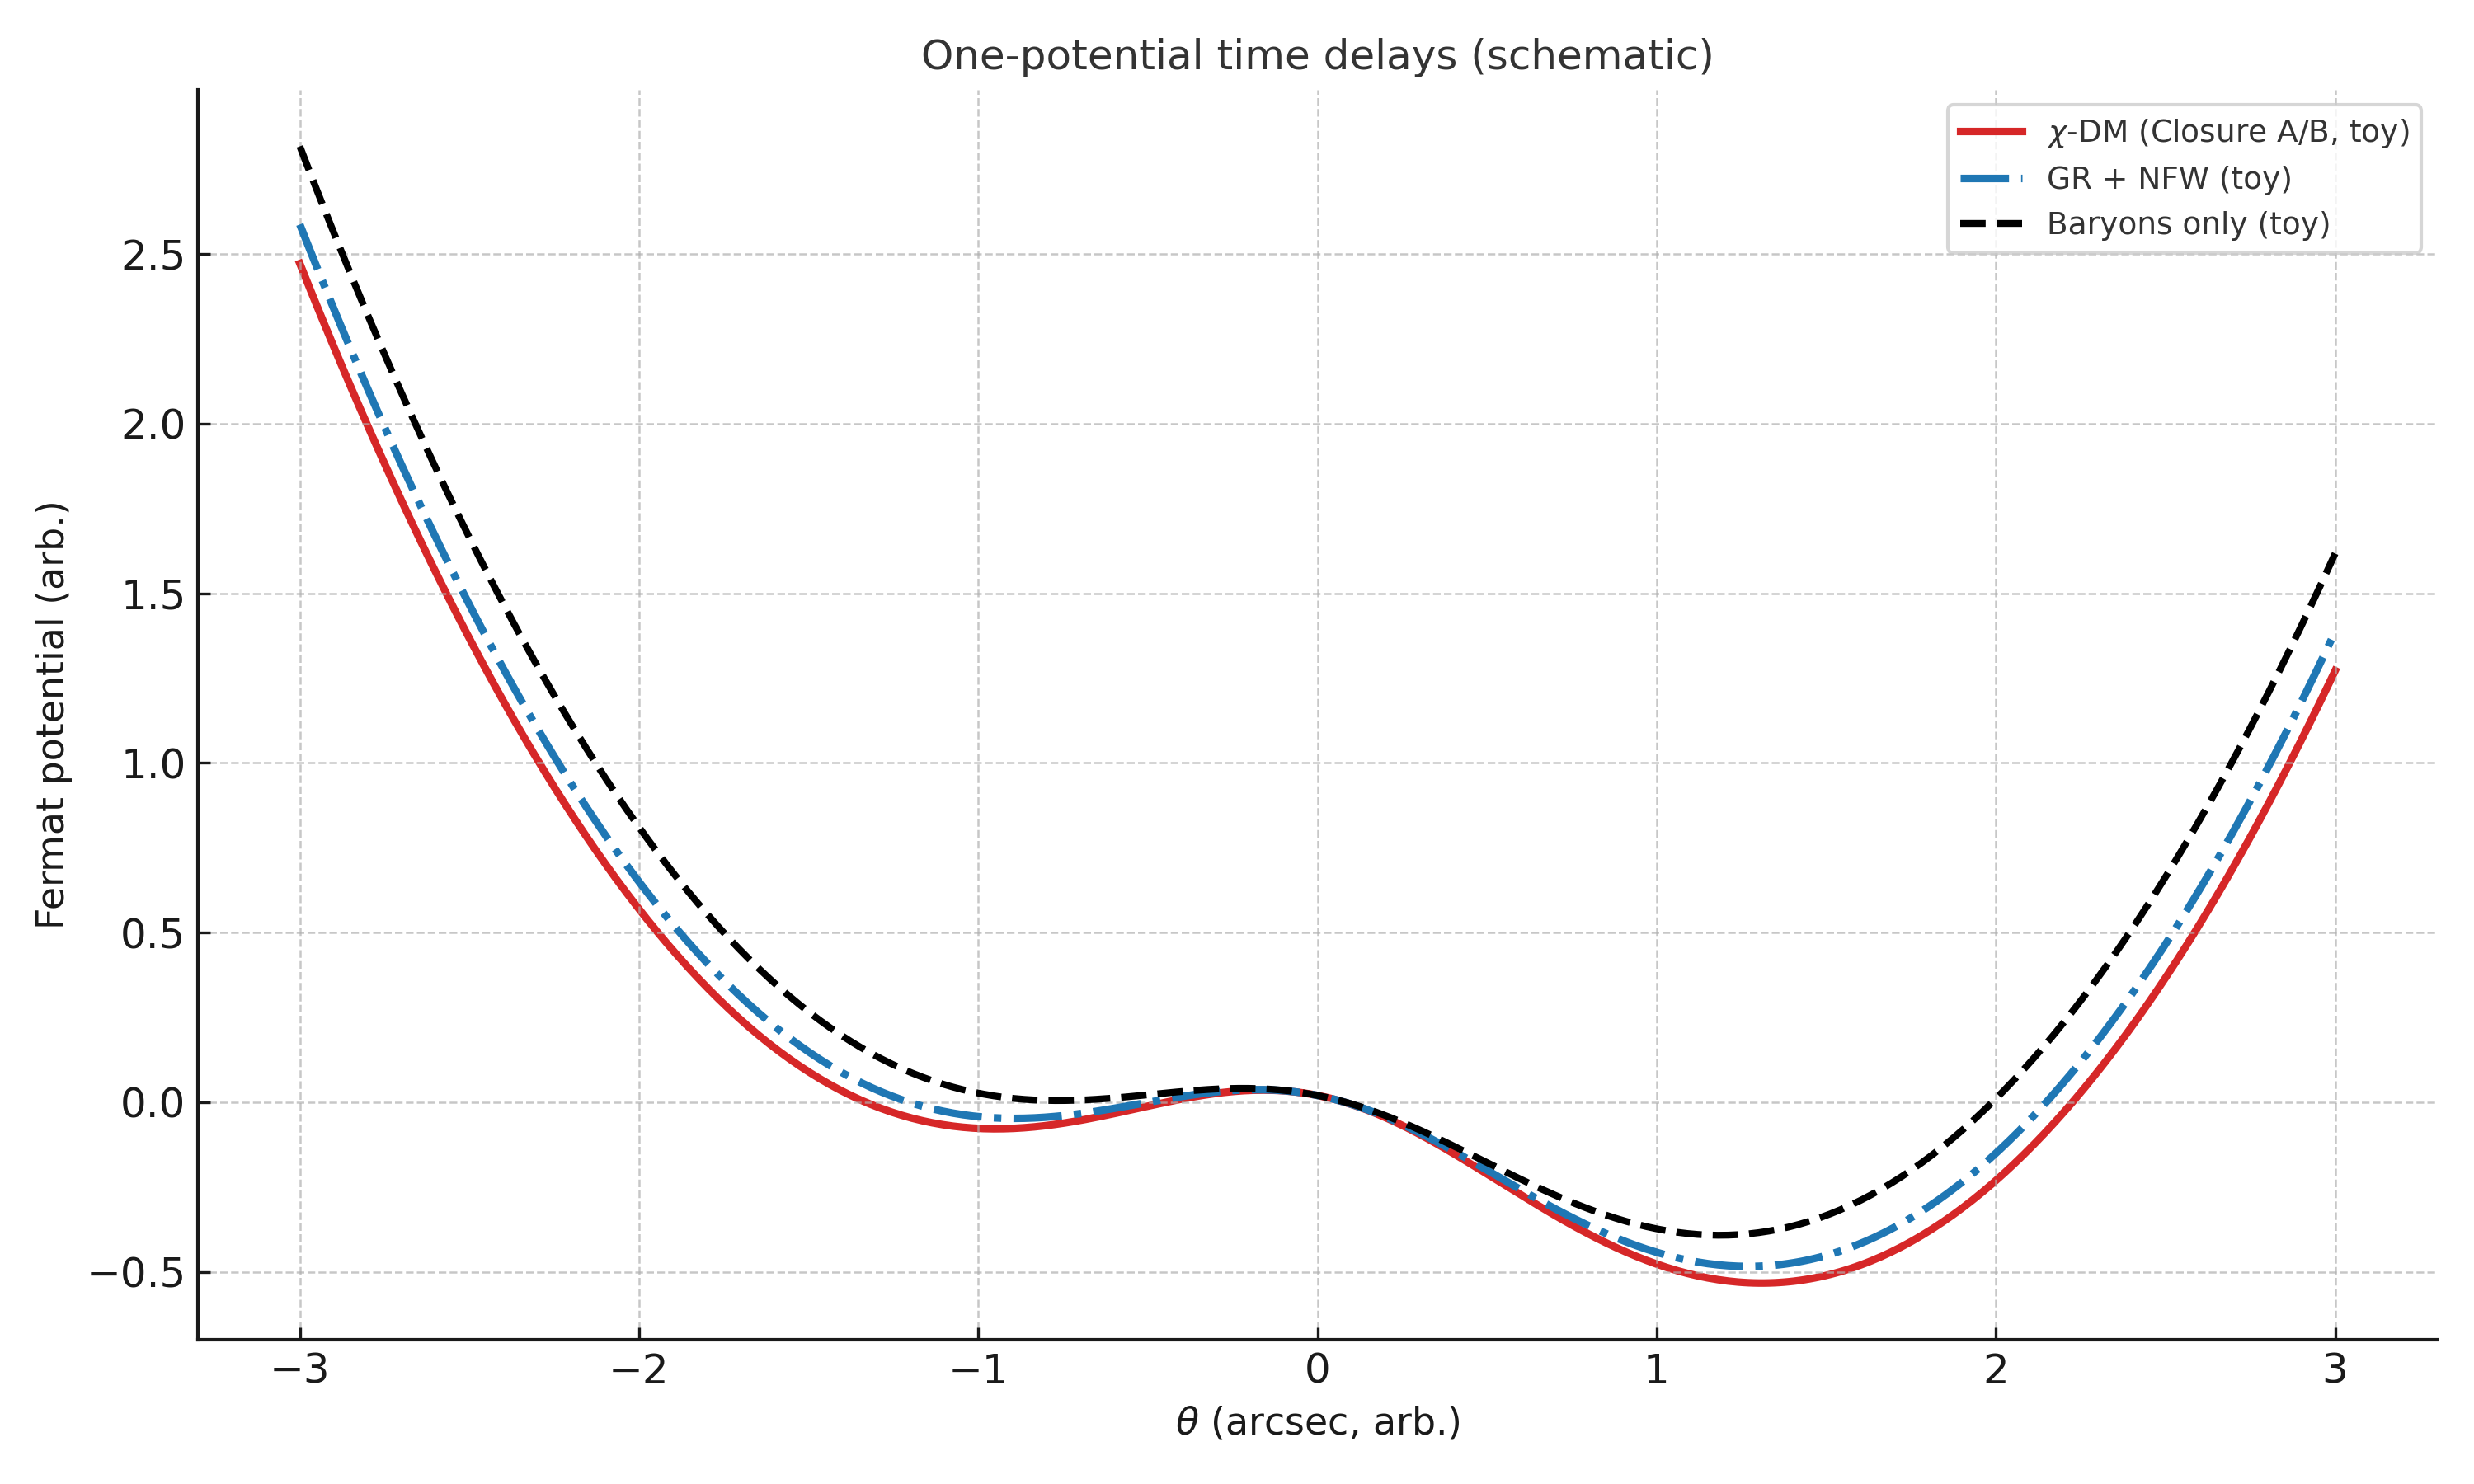
\includegraphics[width=4.01002in,height=2.40601in,alt={A graph of a line graph AI-generated content may be incorrect.}]{letter_media/media/image1.png}

One-potential time delays (schematic). \emph{Sources/assumptions:} Toy
Fermat potential with baryons-only, GR+NFW, and \(\mathbf{\chi}\)-DM
(Closure A/B). The shared \(\mathbf{\Phi}\) deepens minima when
strengthened by a low-acceleration mapping.

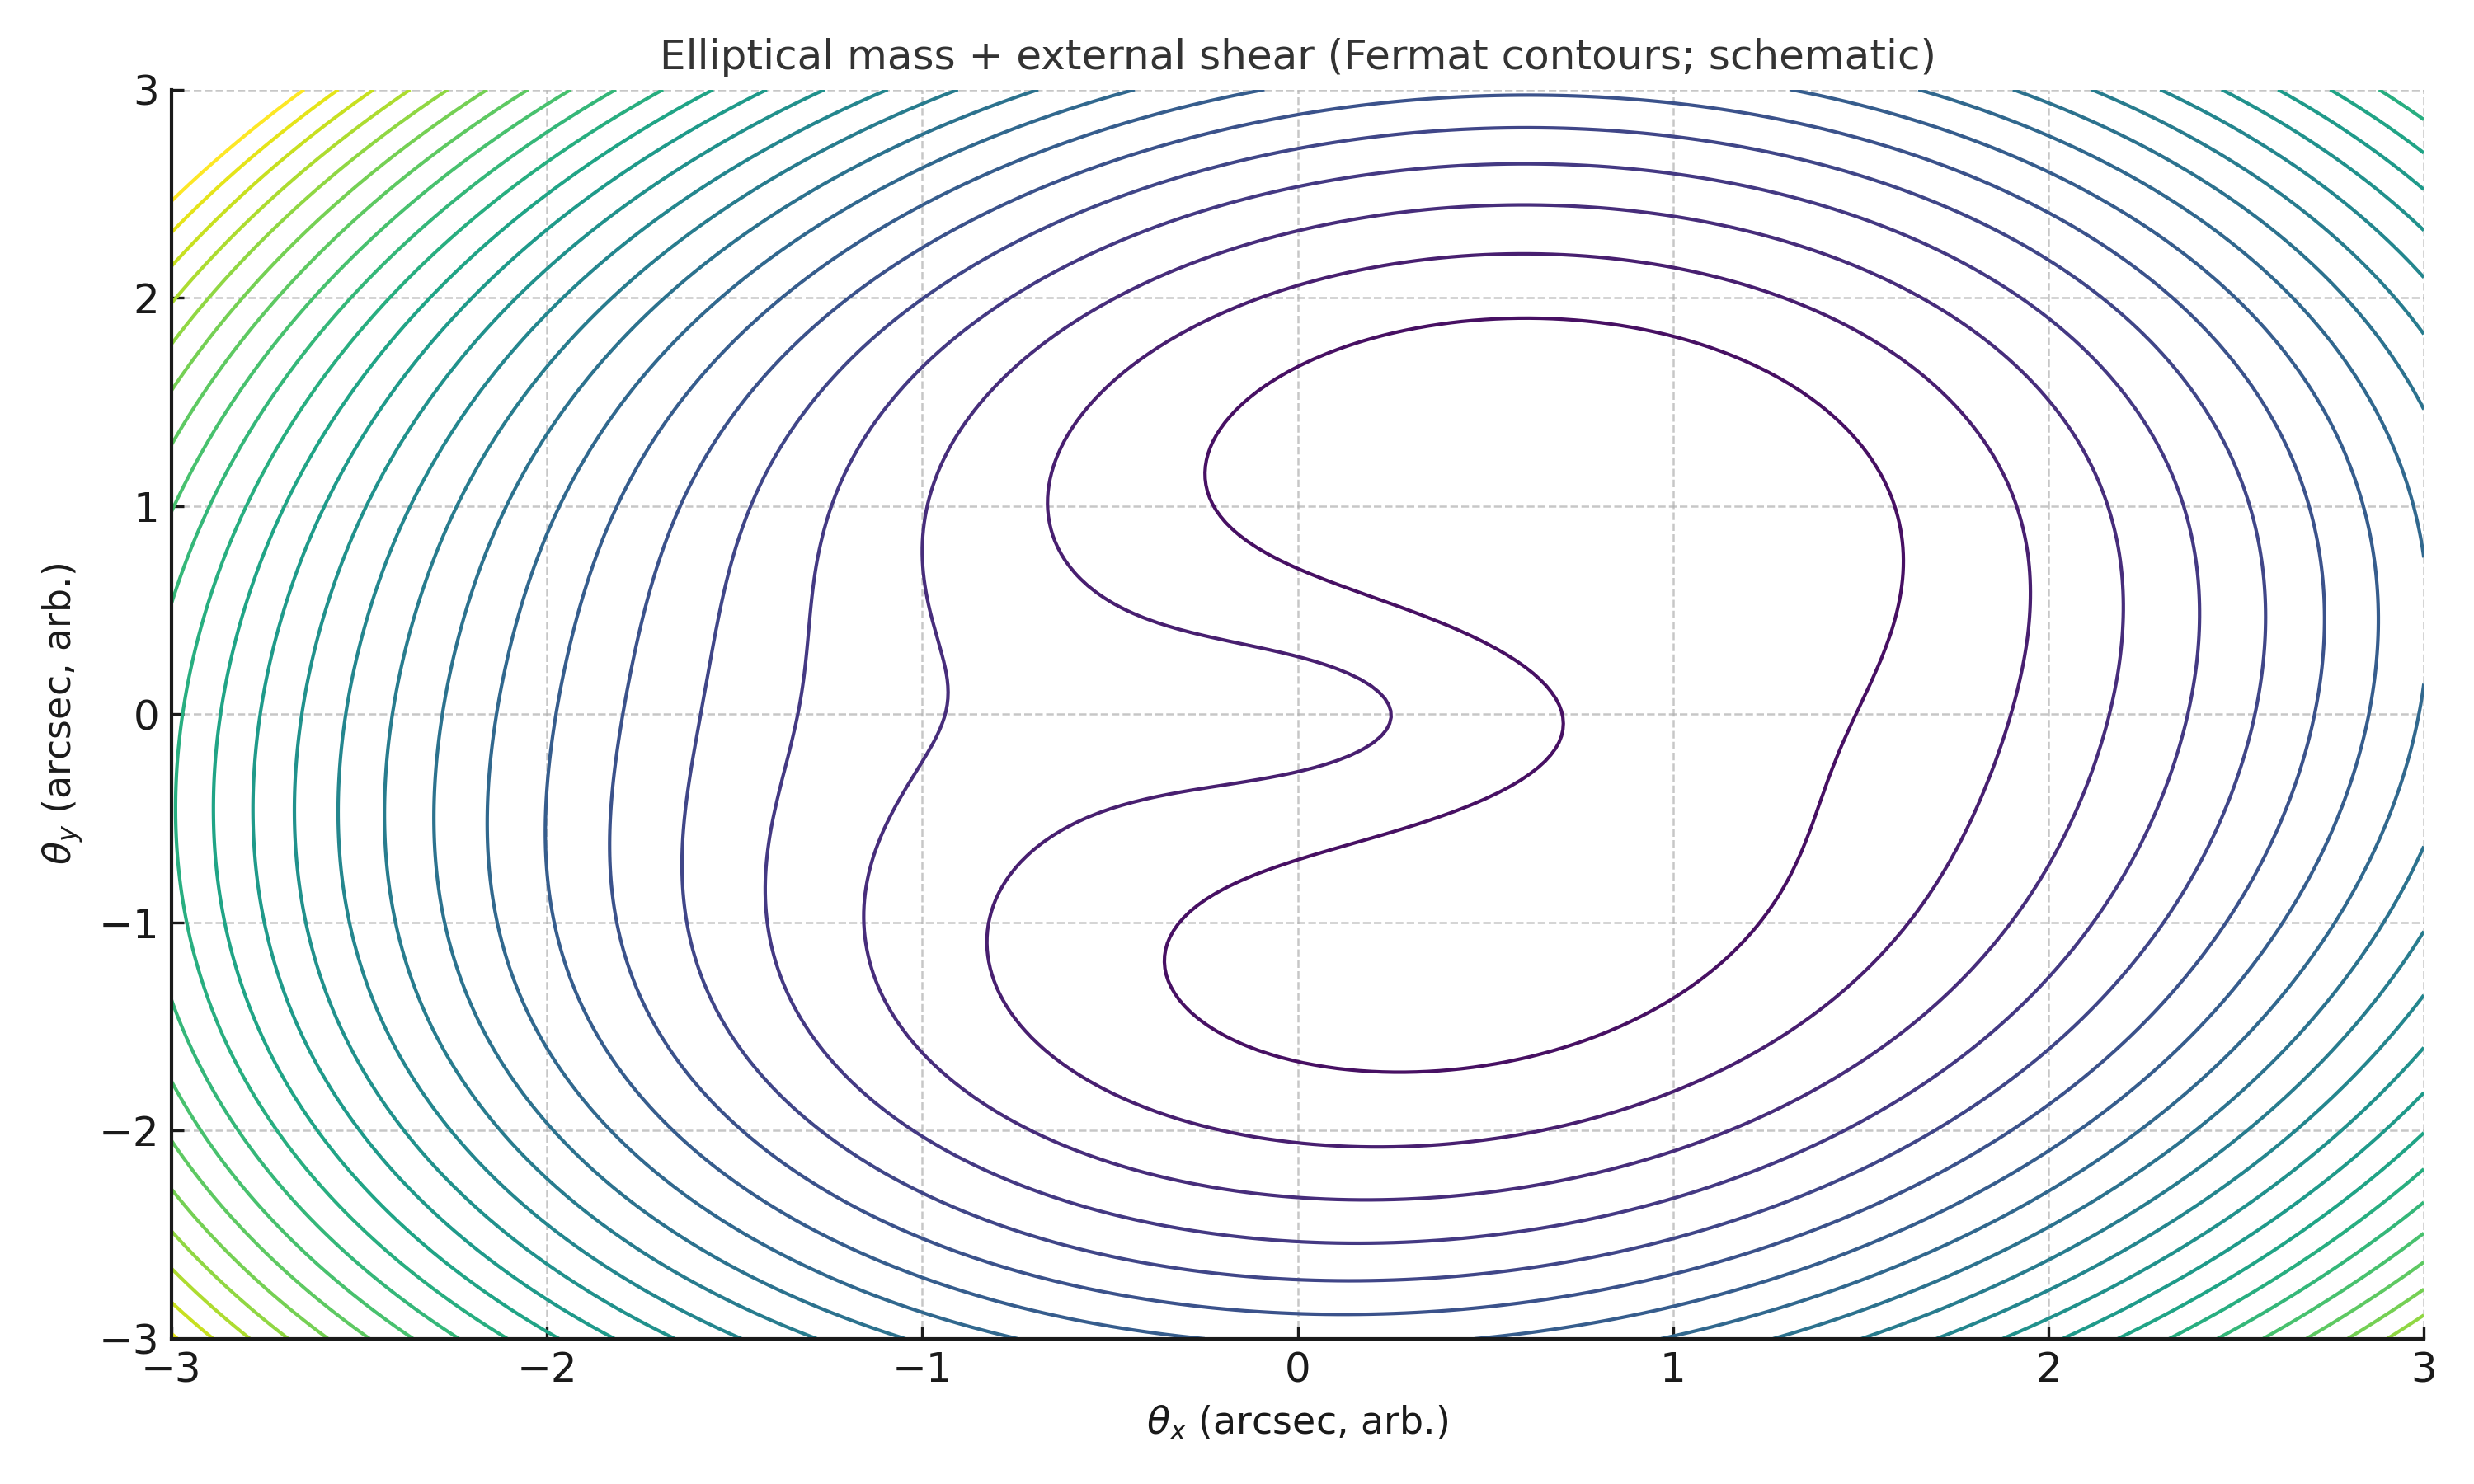
\includegraphics[width=4.05948in,height=2.43569in,alt={A graph of a graph AI-generated content may be incorrect.}]{letter_media/media/image2.png}

Elliptical mass + external shear (Fermat contours; schematic).
\emph{Sources/assumptions:} Elliptical toy potential (softened) plus a
weak external shear rotated by \(\mathbf{30}^{\mathbf{\circ}}\). The
same \(\mathbf{\Phi}\) governs time-delay surfaces and dynamics; optics
keep \(\mathbf{\gamma}\mathbf{=}\mathbf{1}\).

\section{Solar-System safety: numbers and
cross-walk}\label{solar-system-safety-numbers-and-cross-walk}

For the Sun and the simple \(\chi\)-DM mapping used in disk fits, the
fractional acceleration deviation
\(\delta g \equiv |g_{mod} - g_{N}|/g_{N}\) scales roughly like
\(a_{0}/g_{N}\) in the high-acceleration regime. Using
\(a_{0} = 1.1 \times 10^{- 10}\, m/s^{2}\) we obtain the values in the
following table.

\begin{longtable}[]{@{}
  >{\raggedright\arraybackslash}p{(\linewidth - 4\tabcolsep) * \real{0.0998}}
  >{\centering\arraybackslash}p{(\linewidth - 4\tabcolsep) * \real{0.2522}}
  >{\centering\arraybackslash}p{(\linewidth - 4\tabcolsep) * \real{0.6479}}@{}}
\toprule\noalign{}
\begin{minipage}[b]{\linewidth}\raggedright
\textbf{Radius}
\end{minipage} & \begin{minipage}[b]{\linewidth}\centering
\(\mathbf{\delta g}\) (baseline mapping)
\end{minipage} & \begin{minipage}[b]{\linewidth}\centering
\textbf{Comment}
\end{minipage} \\
\midrule\noalign{}
\endhead
\bottomrule\noalign{}
\endlastfoot
\(1\) AU & \(\sim 2 \times 10^{- 8}\) & Deep in high-\(g\) regime;
essentially Newtonian/GR. \\
\(10\) AU & \(\sim 2 \times 10^{- 6}\) & Well within standard navigation
tolerances. \\
\(100\) AU & \(\sim 2 \times 10^{- 4}\) & Outer-heliospheric scale; for
future ephemeris cross-checks. \\
\end{longtable}

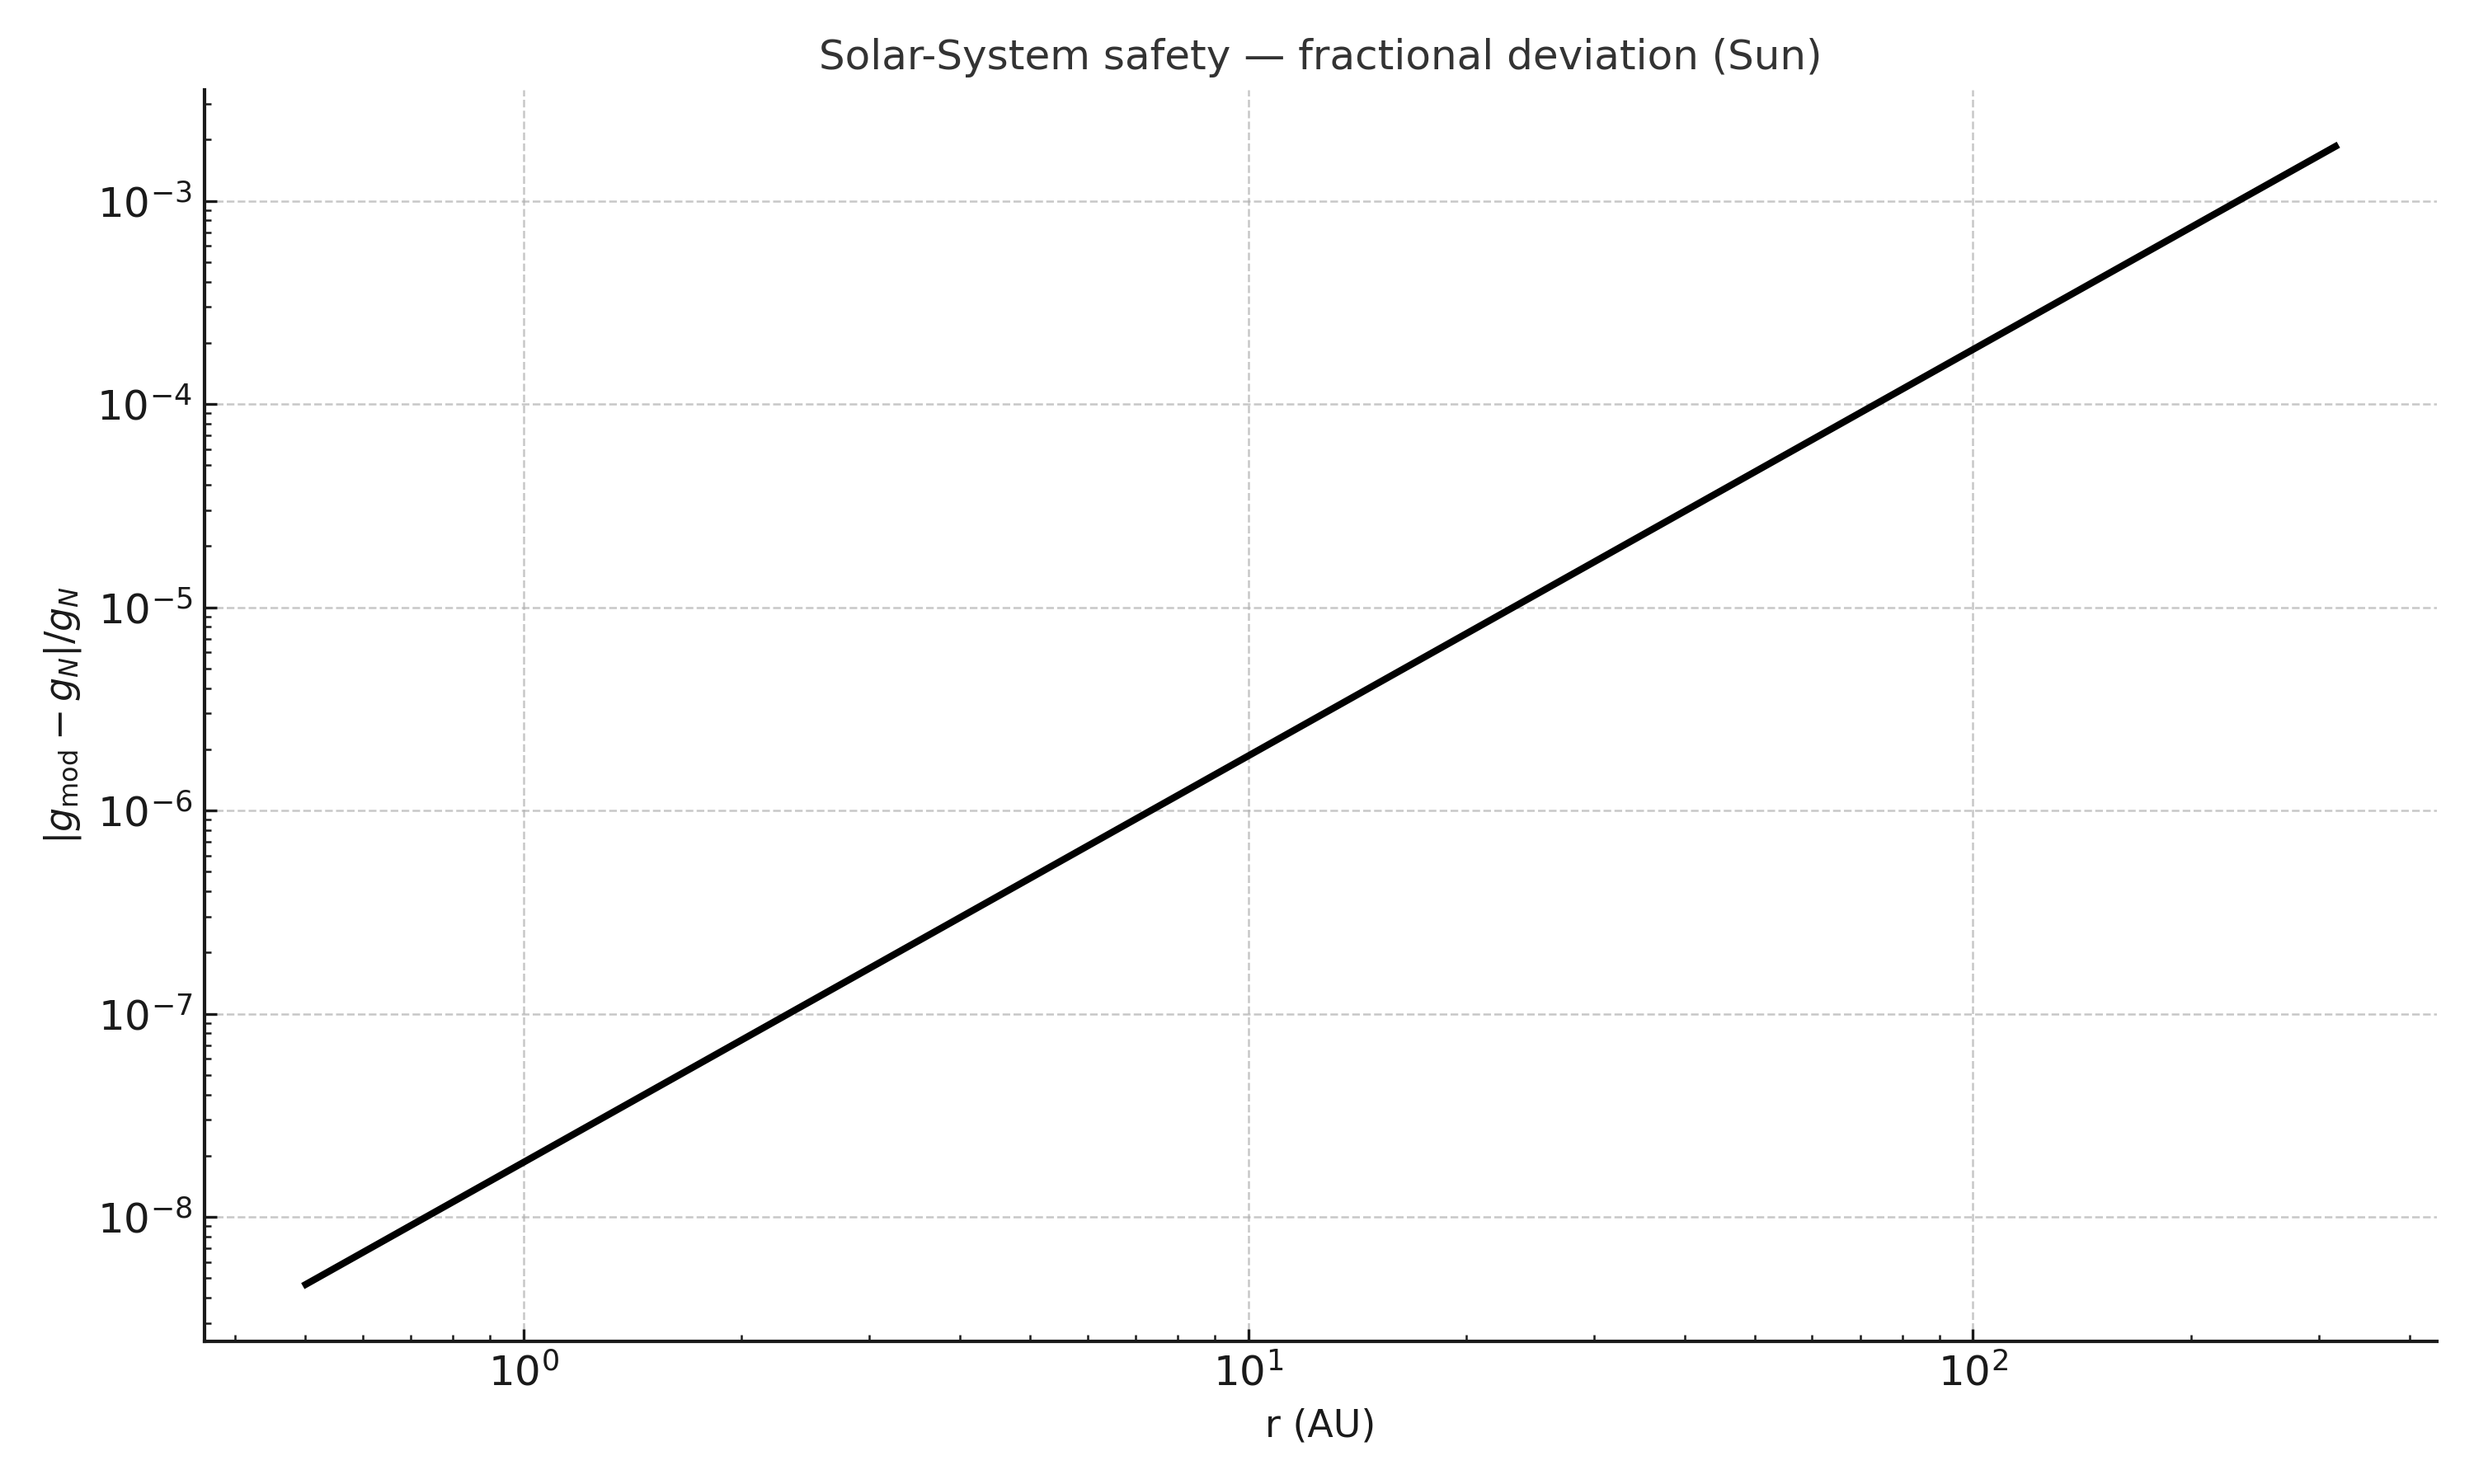
\includegraphics[width=4.78333in,height=2.87in,alt={A graph with a line AI-generated content may be incorrect.}]{letter_media/media/image3.png}

Solar-System safety. \emph{Sources/assumptions:} Sun as a monopole;
\(\mathbf{\chi}\)-DM mapping applied to the Newtonian field. Shown is
the fractional deviation
\(\mathbf{|}\mathbf{g}_{\mathbf{mod}}\mathbf{-}\mathbf{g}_{\mathbf{N}}\mathbf{|/}\mathbf{g}_{\mathbf{N}}\)
vs \(\mathbf{r}\).

\section{\texorpdfstring{Monte-Carlo calibration: kernel, window, and
per-\(\alpha\)
results}{Monte-Carlo calibration: kernel, window, and per-\textbackslash alpha results}}\label{monte-carlo-calibration-kernel-window-and-per-alpha-results}

We use the near-side, gauge-safe LOS functional so that
\(\Delta H/H_{0} = \alpha\,\bar{I}\). The window \(W(s)\) is normalized;
magnitude-kernel rows are included for comparison.

\begin{longtable}[]{@{}
  >{\raggedright\arraybackslash}p{(\linewidth - 6\tabcolsep) * \real{0.3266}}
  >{\centering\arraybackslash}p{(\linewidth - 6\tabcolsep) * \real{0.2245}}
  >{\centering\arraybackslash}p{(\linewidth - 6\tabcolsep) * \real{0.2245}}
  >{\centering\arraybackslash}p{(\linewidth - 6\tabcolsep) * \real{0.2245}}@{}}
\toprule\noalign{}
\begin{minipage}[b]{\linewidth}\raggedright
\textbf{Environment \& kernel}
\end{minipage} & \begin{minipage}[b]{\linewidth}\centering
\textbf{median(}\(\bar{I}\)\textbf{)}
\end{minipage} & \begin{minipage}[b]{\linewidth}\centering
\[\mathbf{p}_{\mathbf{16}}\]
\end{minipage} & \begin{minipage}[b]{\linewidth}\centering
\[\mathbf{p}_{\mathbf{84}}\]
\end{minipage} \\
\midrule\noalign{}
\endhead
\bottomrule\noalign{}
\endlastfoot
Cluster --- near-side & \(- 1.885 \times 10^{- 6}\) &
\(- 3.370 \times 10^{- 6}\) & \(- 1.353 \times 10^{- 6}\) \\
Void --- near-side & \(+ 6.292 \times 10^{- 7}\) &
\(+ 1.226 \times 10^{- 7}\) & \(+ 4.498 \times 10^{- 6}\) \\
Cluster --- magnitude & \(+ 3.770 \times 10^{- 6}\) &
\(+ 2.685 \times 10^{- 6}\) & \(+ 6.804 \times 10^{- 6}\) \\
Void --- magnitude & \(+ 1.564 \times 10^{- 6}\) &
\(+ 4.091 \times 10^{- 7}\) & \(+ 9.660 \times 10^{- 6}\) \\
\end{longtable}

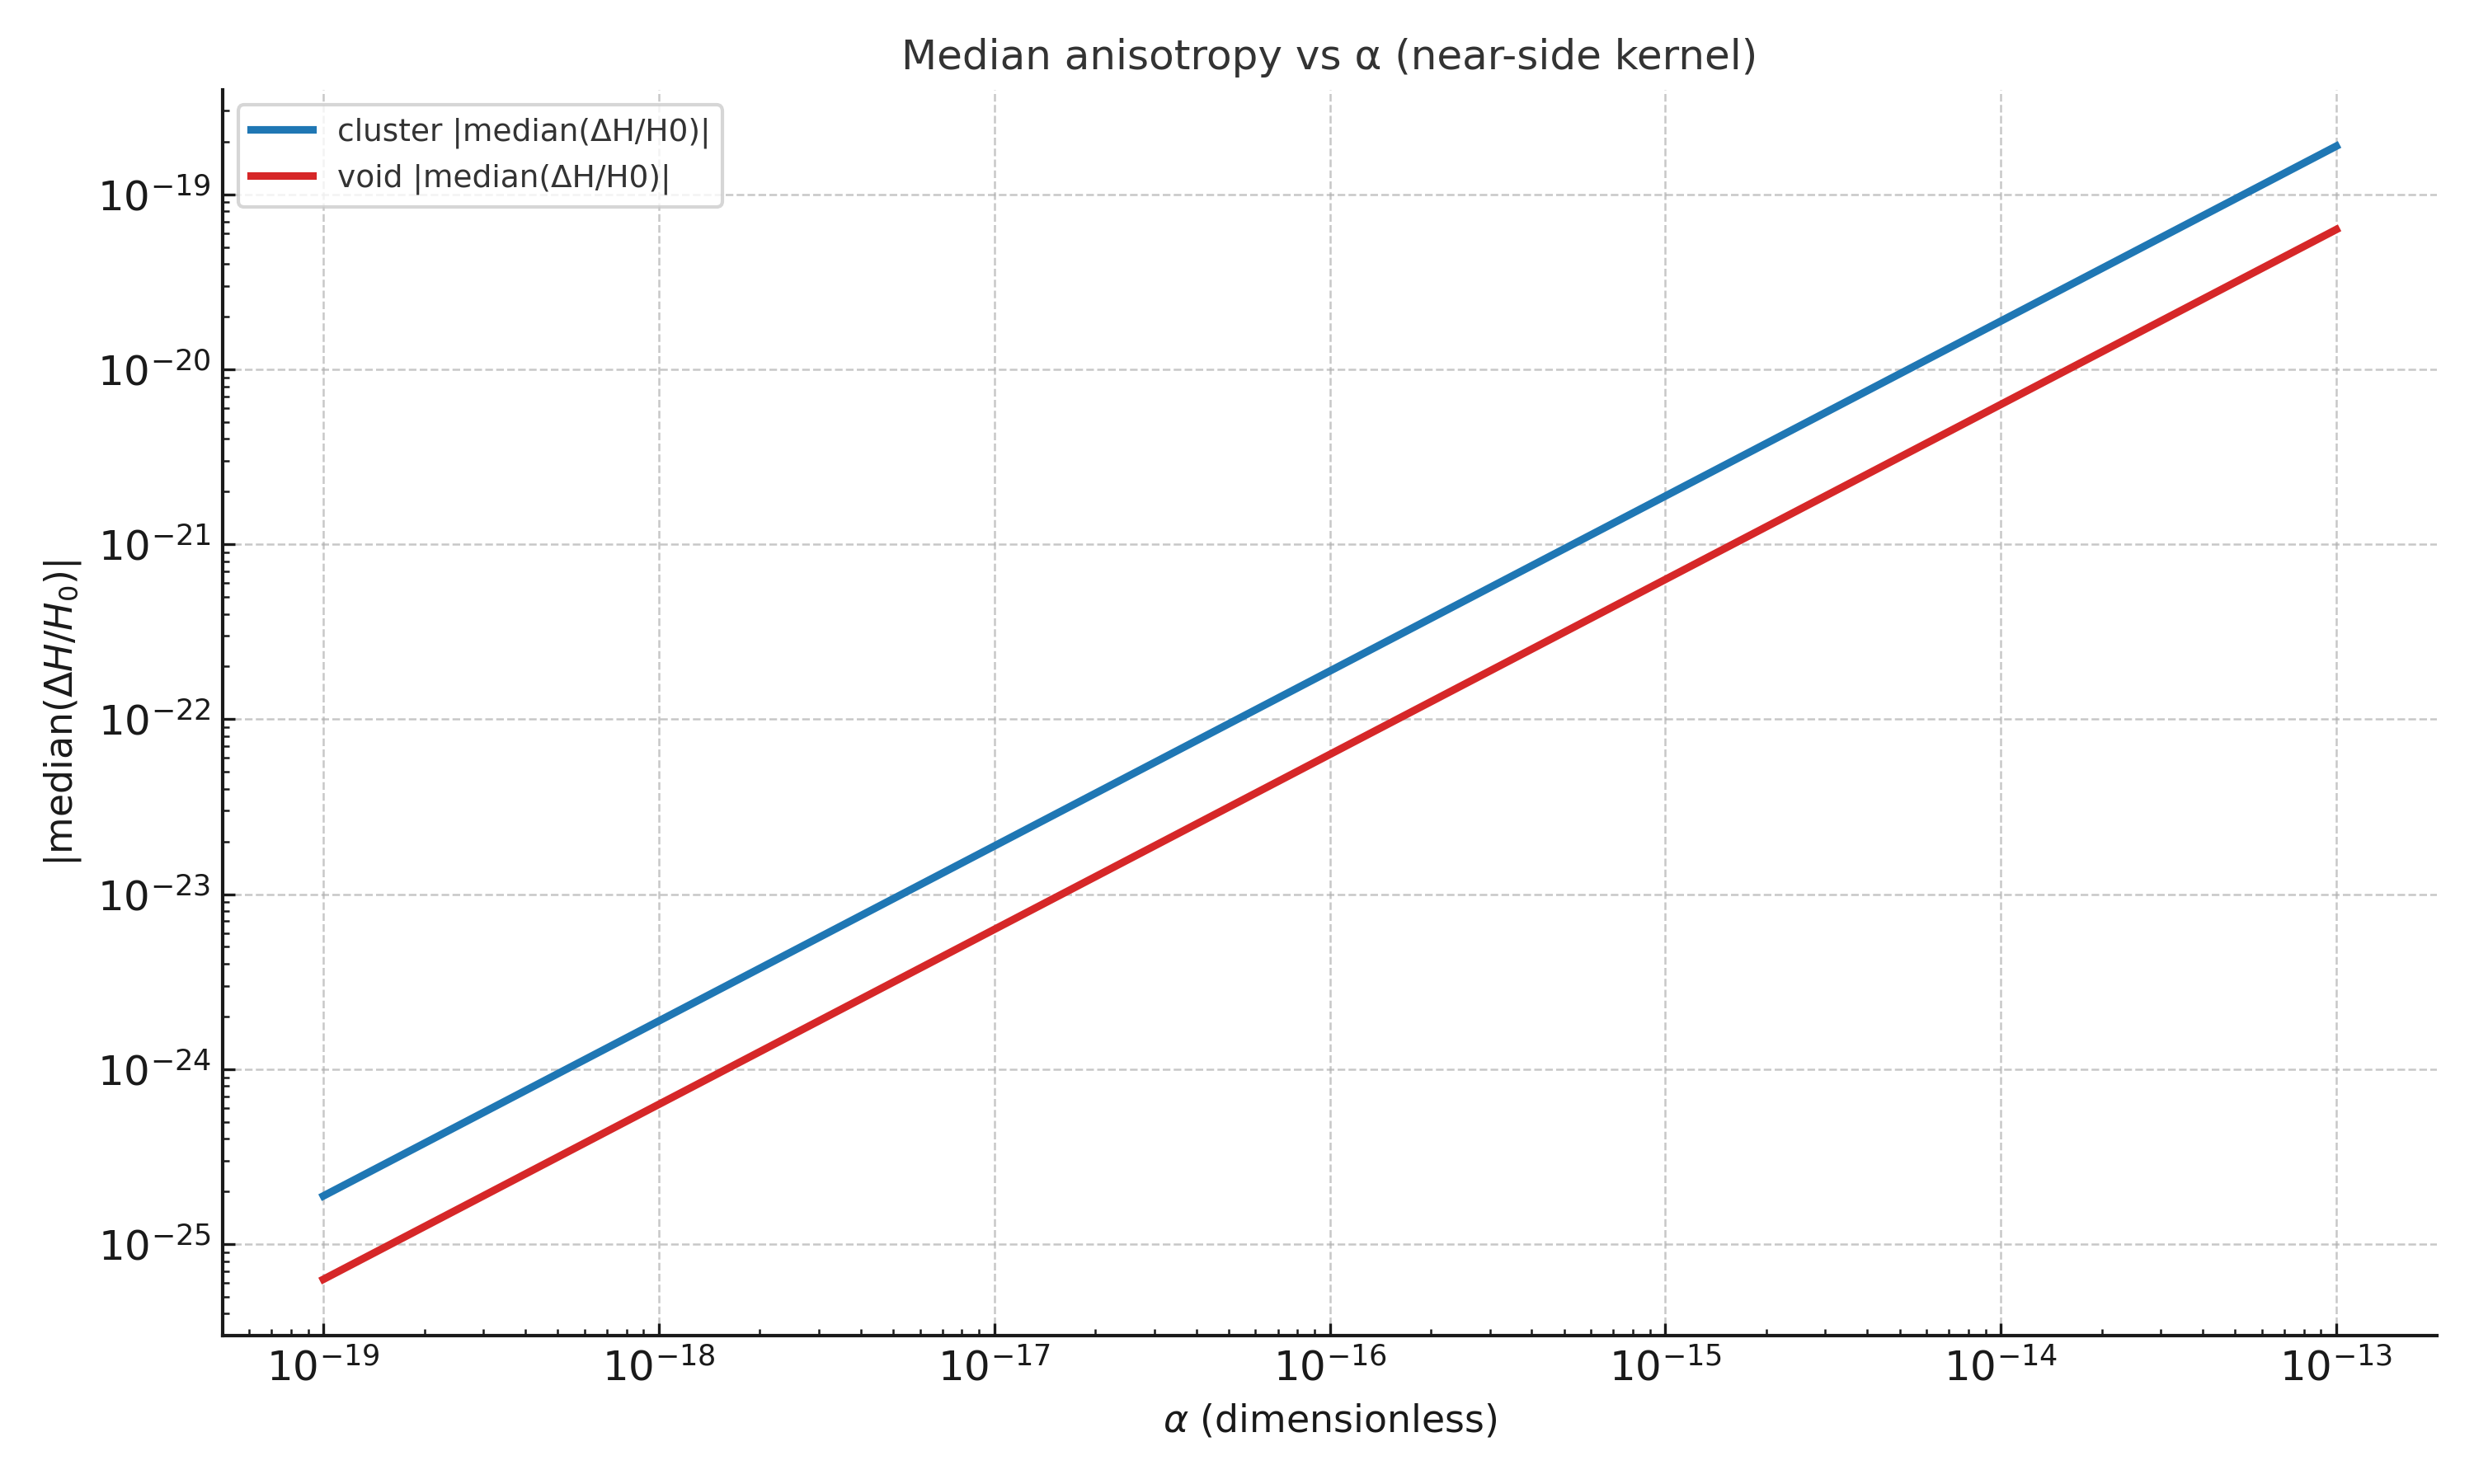
\includegraphics[width=4.78333in,height=2.87in,alt={A graph with a red line AI-generated content may be incorrect.}]{letter_media/media/image4.png}

Median anisotropy
\(\mathbf{|median(\Delta}\mathbf{H}\mathbf{/}\mathbf{H}_{\mathbf{0}}\mathbf{)|}\)
vs \(\mathbf{\alpha}\) (near-side kernel). \emph{Sources/assumptions:}
synthetic Monte Carlo using a unit-normalized window; Linear scaling
with \(\mathbf{\alpha}\) is evident.

\section{\texorpdfstring{Notation standardization \& \(\nu\)--\(\mu\)
table}{Notation standardization \& \textbackslash nu--\textbackslash mu table}}\label{notation-standardization-numu-table}

We use \(\chi\)\emph{-DM} for the low-acceleration mapping with one
global \(a_{0}\).

The interpolating/fade-out function is denoted \(\mu( \cdot )\); any
future high-\(g\) taper will be written as \(\mu_{hi}(g_{b}/a_{0})\)
(not \(\nu\)).

\begin{longtable}[]{@{}
  >{\raggedright\arraybackslash}p{(\linewidth - 4\tabcolsep) * \real{0.1243}}
  >{\raggedright\arraybackslash}p{(\linewidth - 4\tabcolsep) * \real{0.5231}}
  >{\raggedright\arraybackslash}p{(\linewidth - 4\tabcolsep) * \real{0.3527}}@{}}
\toprule\noalign{}
\begin{minipage}[b]{\linewidth}\raggedright
Symbol
\end{minipage} & \begin{minipage}[b]{\linewidth}\raggedright
Meaning
\end{minipage} & \begin{minipage}[b]{\linewidth}\raggedright
Baseline form
\end{minipage} \\
\midrule\noalign{}
\endhead
\bottomrule\noalign{}
\endlastfoot
\(\mu(y)\) & source-side interpolation with \(y \equiv g/a_{0}\) &
\(\mu(y) = \frac{y}{1 + y}\) \\
\(\nu(y_{b})\) & field-side response with \(y_{b} \equiv g_{b}/a_{0}\) &
\(\nu(y_{b}) = \frac{1}{2}\left( 1 + \sqrt{1 + \frac{4}{y_{b}}} \right)\) \\
\end{longtable}

\section{Related work (brief,
non-exhaustive)}\label{related-work-brief-non-exhaustive-1}

Expansion-based or emergent-gravity intuitions have appeared before,
notably in work by Erik Verlinde (entropic/emergent gravity) and Mark
McCutcheon (expansion-based ideas). There are also modified-gravity
frameworks such as MOND/TeVeS, MOG, and \(f(R)\). The present letter is
conservative: it keeps GR's tested optics (\(\gamma = 1\)), enforces one
shared \(\Phi\) for motion \emph{and} lensing/time delays, and states
falsifiers upfront.\footnote{Consistency with our published 2-page
  explainer is intentional: same mapping \(\Phi \equiv c^{2}\chi\), same
  classic tests and falsifiers.}

\section{Acknowledgements}\label{acknowledgements}

We thank early readers and colleagues; maintainers of open-source tools;
and the ephemeris, precision clock, gravitational-wave, and
large-scale-structure communities whose public results constrain our
safe-regime choices. We thank OpenAI for the wizardry behind ChatGPT. We
are grateful to \textbf{Zé Ayala}, \textbf{Robert Ryan}, \textbf{Joon
Yun}, and \textbf{Mariano Muñoz} for inspiring conversations, and we
thank the human author's family for their endless support and
encouragement. Any errors remain our own.

\section{Appendix A: Exponential-disk rotation curve
(formula)}\label{appendix-a-exponential-disk-rotation-curve-formula}

For a thin exponential disk with surface density
\(\Sigma(R) = \Sigma_{0}e^{- R/R_{d}}\) and
\(\Sigma_{0} = M_{d}/(2\pi R_{d}^{2})\), the circular speed is

\[v_{c}^{2}(R) = 4\pi G\Sigma_{0}R_{d}\, y^{2}\,\lbrack I_{0}(y)K_{0}(y) - I_{1}(y)K_{1}(y)\rbrack,\quad\quad y \equiv \frac{R}{2R_{d}},\]

with modified Bessel functions \(I_{n}\) and \(K_{n}\).

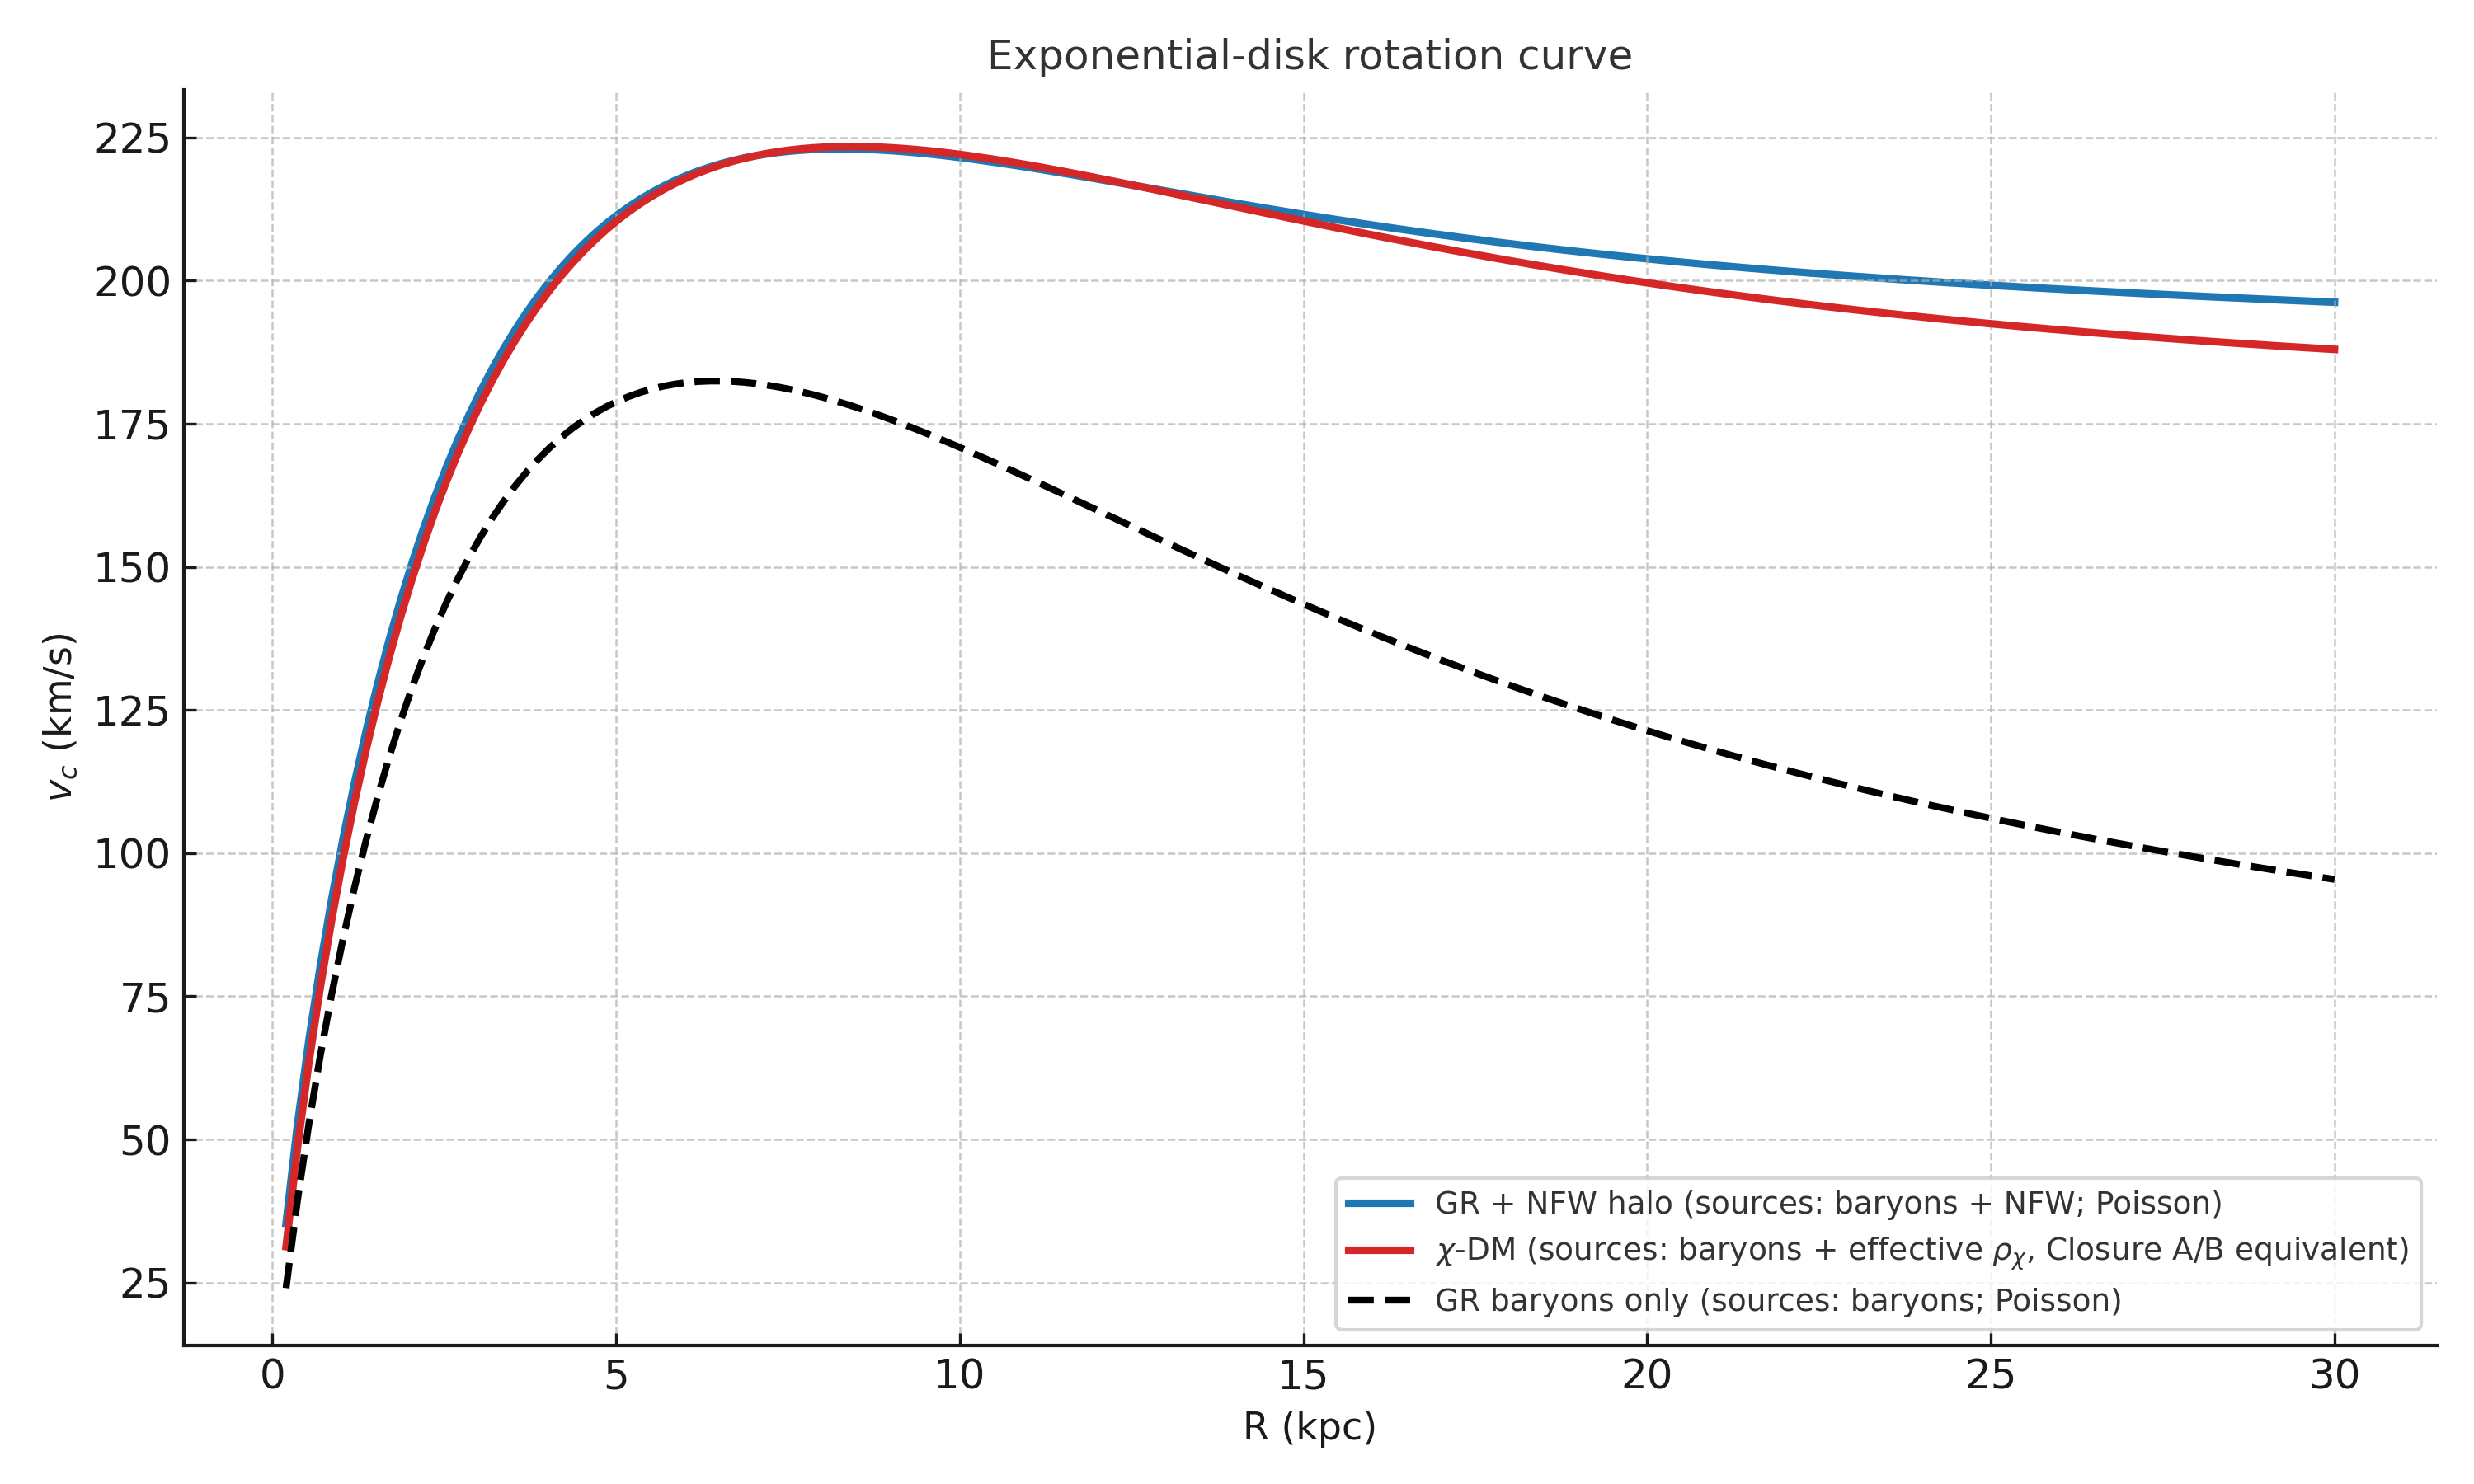
\includegraphics[width=4.78333in,height=2.87in,alt={A graph of a graph of a number of different colored lines AI-generated content may be incorrect.}]{letter_media/media/image5.png}

Exponential-disk rotation curve. \emph{Sources used:} GR baryons only
(Poisson); GR+NFW (baryons+NFW); \(\mathbf{\chi}\)-DM
\(\mathbf{\equiv}\) baryons + effective
\(\mathbf{\rho}_{\mathbf{\chi}}\) (Closure A/B). \emph{Styles:} GR+NFW
(blue solid), \(\mathbf{\chi}\)-DM (red solid), GR baryons only (black
dashed, overlaid).

\section{Appendix B: Hernquist lens --- deflection from one
potential}\label{appendix-b-hernquist-lens-deflection-from-one-potential}

Consider a spherical Hernquist profile with total baryonic mass \(M\)
and scale \(a\). The baryonic gravitational acceleration is

\[g_{b}(r)\mspace{6mu} = \mspace{6mu}\frac{GM}{(r + a)^{2}}.\]

With the baseline low-\(g\) mapping (``\(\chi\)-DM'') we use

\[g(r)\mspace{6mu} = \mspace{6mu}\frac{1}{2}\left\lbrack g_{b}(r) + \sqrt{g_{b}(r)^{2} + 4\, g_{b}(r)\, a_{0}} \right\rbrack,\]

and define the potential by \(\partial_{r}\Phi = g(r)\). For an
axisymmetric thin lens with cylindrical impact parameter \(R\) the
deflection can be written in either of two equivalent one-potential
forms,

\[\alpha(R)\mspace{6mu} = \mspace{6mu}\frac{2}{c^{2}}\int_{- \infty}^{\infty}\frac{\partial\Phi}{\partial R}(R,z)\, dz\mspace{6mu} = \mspace{6mu}\frac{2}{c^{2}}\int_{- \infty}^{\infty}g(r)\,\frac{R}{r}\, dz,\quad\quad r \equiv \sqrt{R^{2} + z^{2}}.\]

\emph{Implementation note.} In our code we evaluate the \(z\)-integral
numerically (adaptive quadrature) using the \(\partial_{R}\Phi\) form
above; this keeps motion and optics tied to the same \(\Phi\) by
construction. The expression reduces to the standard projected-mass
result when \(g \rightarrow g_{b}\) (baryons only). For GR+NFW
comparisons we use

\[g(r)\mspace{6mu} = \mspace{6mu} g_{b}(r) + g_{NFW}(r),\quad\quad g_{NFW}(r)\mspace{6mu} = \mspace{6mu}\frac{G\, M_{NFW}( < r)}{r^{2}},\]

with the usual \(M_{200}\) and concentration parameters defining
\(M_{NFW}( < r)\).

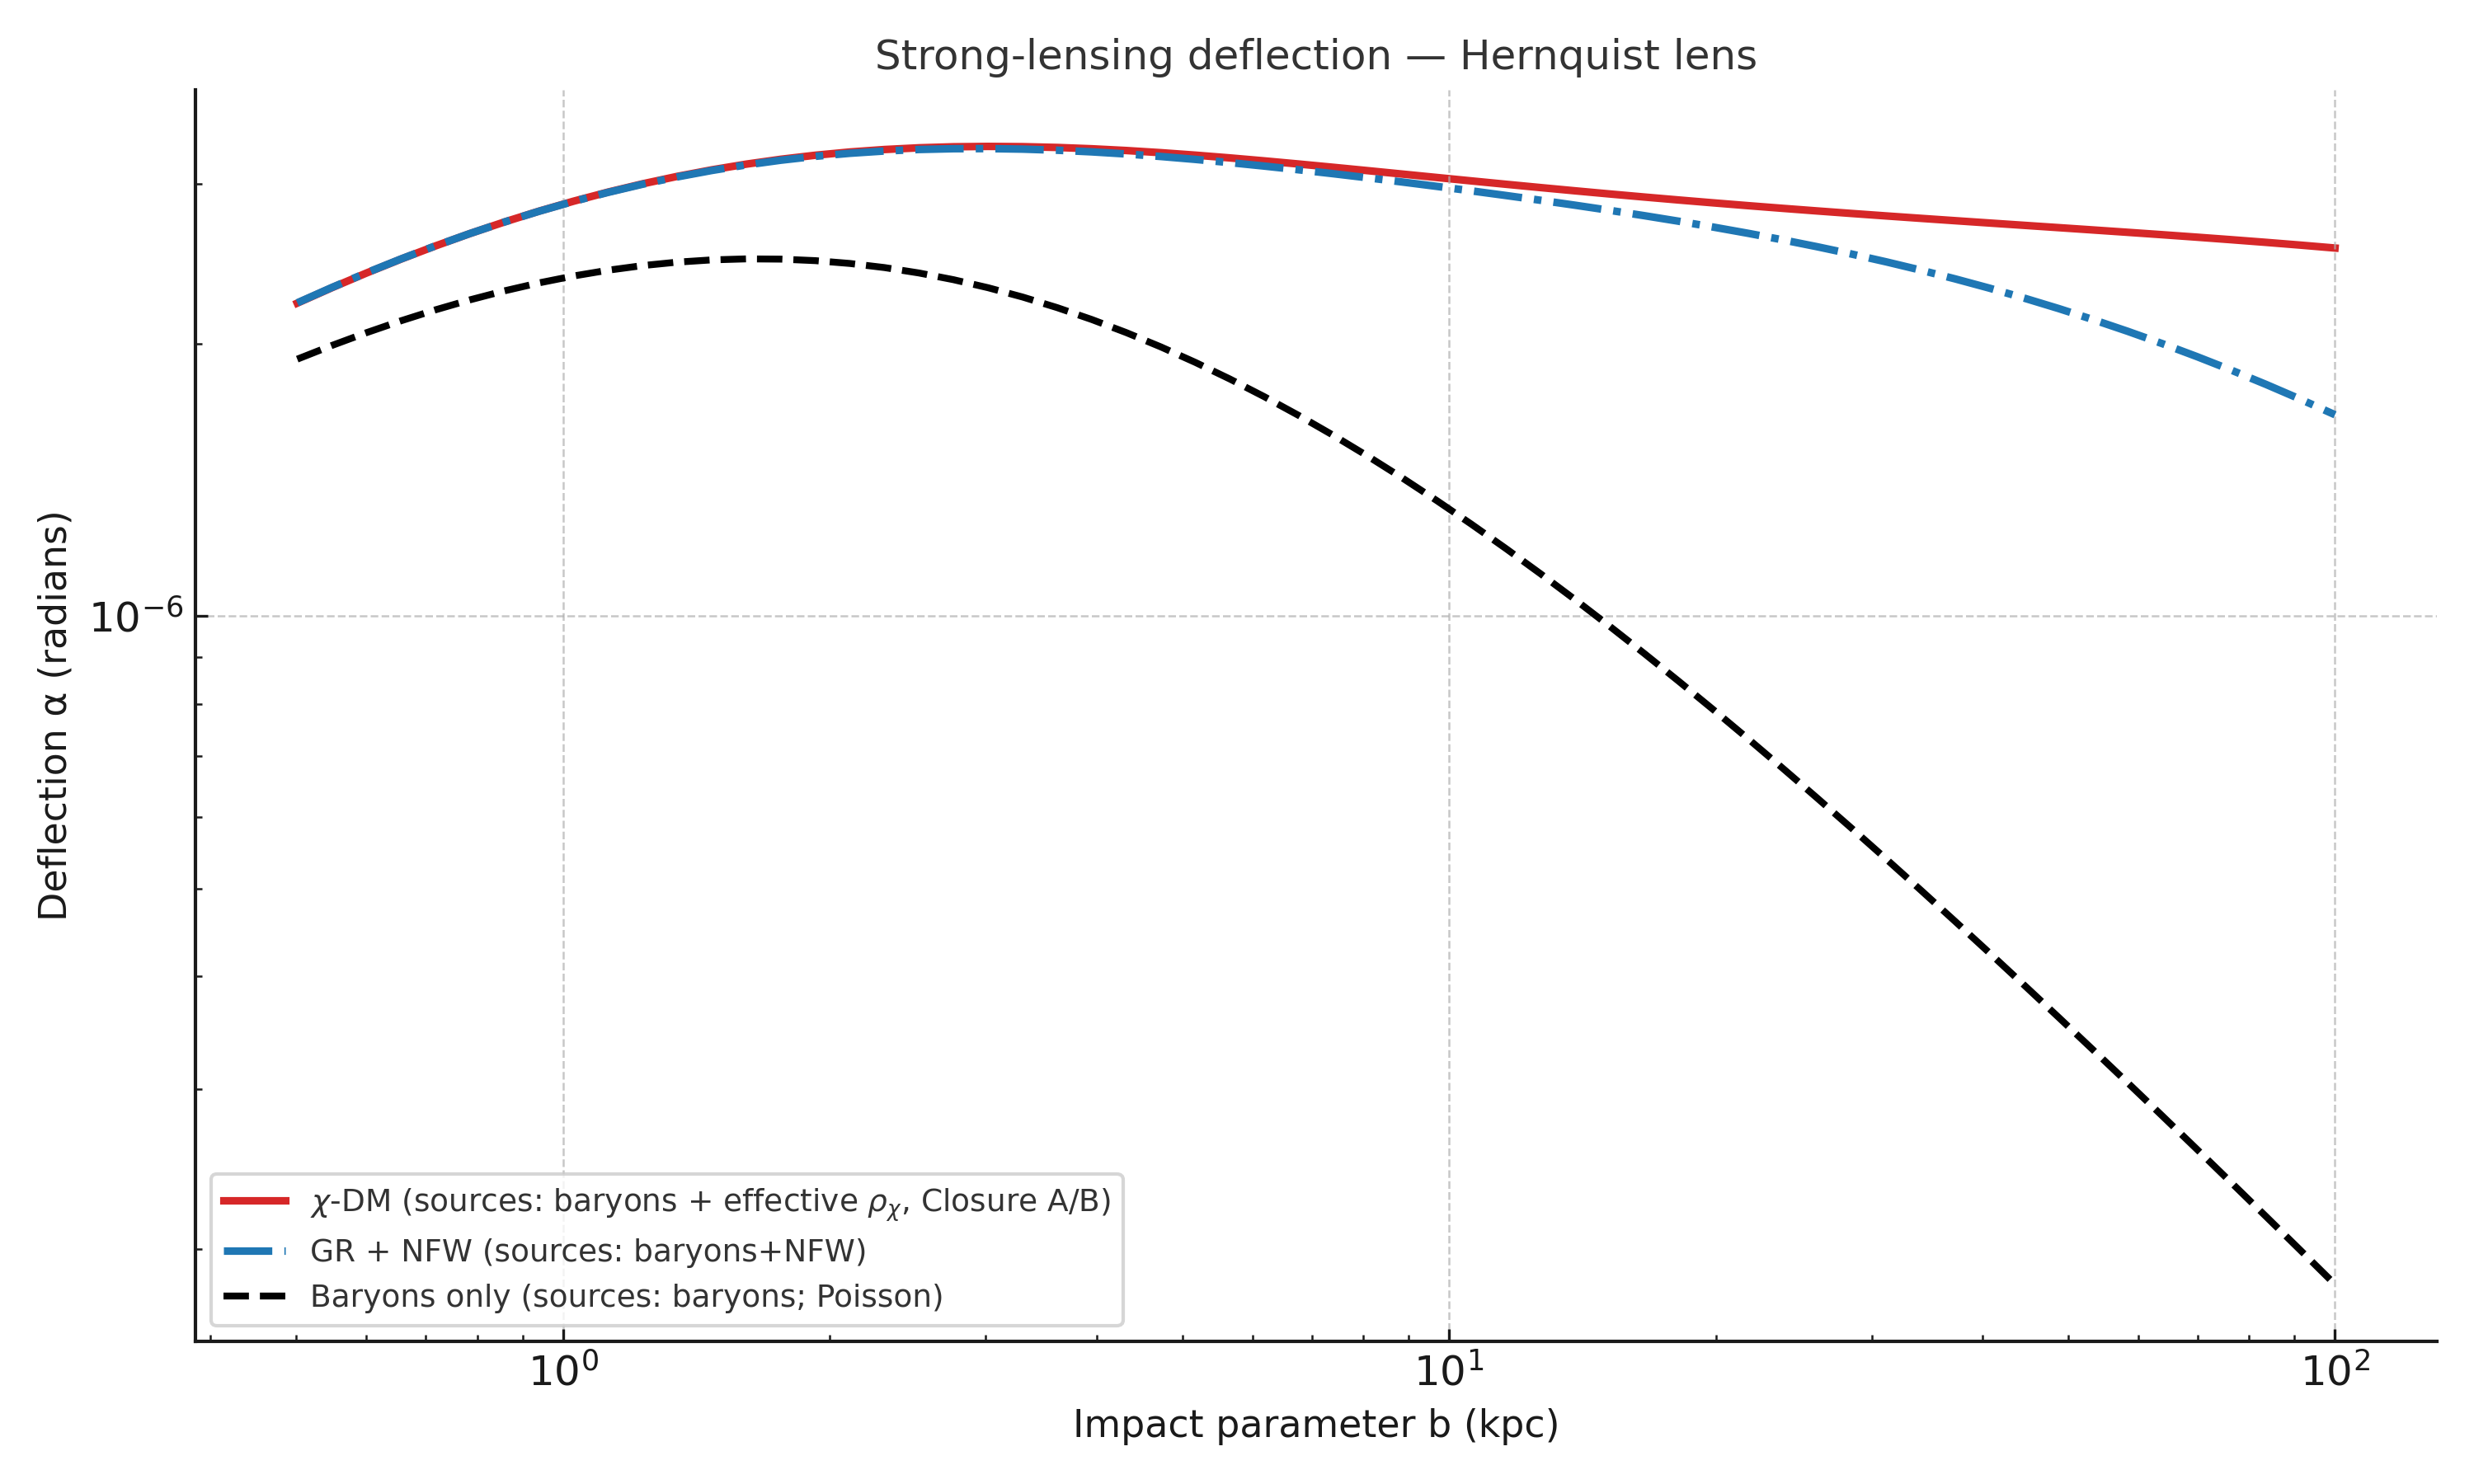
\includegraphics[width=4.78333in,height=2.87in,alt={A graph of a graph AI-generated content may be incorrect.}]{letter_media/media/image6.png}

Strong-lensing deflection for a Hernquist baryonic lens. \emph{Sources
used:} Baryons-only (Poisson), GR+NFW (baryons+NFW),
\(\mathbf{\chi}\)-DM \(\mathbf{\equiv}\) baryons + effective
\(\mathbf{\rho}_{\mathbf{\chi}}\) (Closure A/B). Optics keep
\(\mathbf{\gamma}\mathbf{=}\mathbf{1}\) with the same \(\mathbf{\Phi}\)
for light and motion.

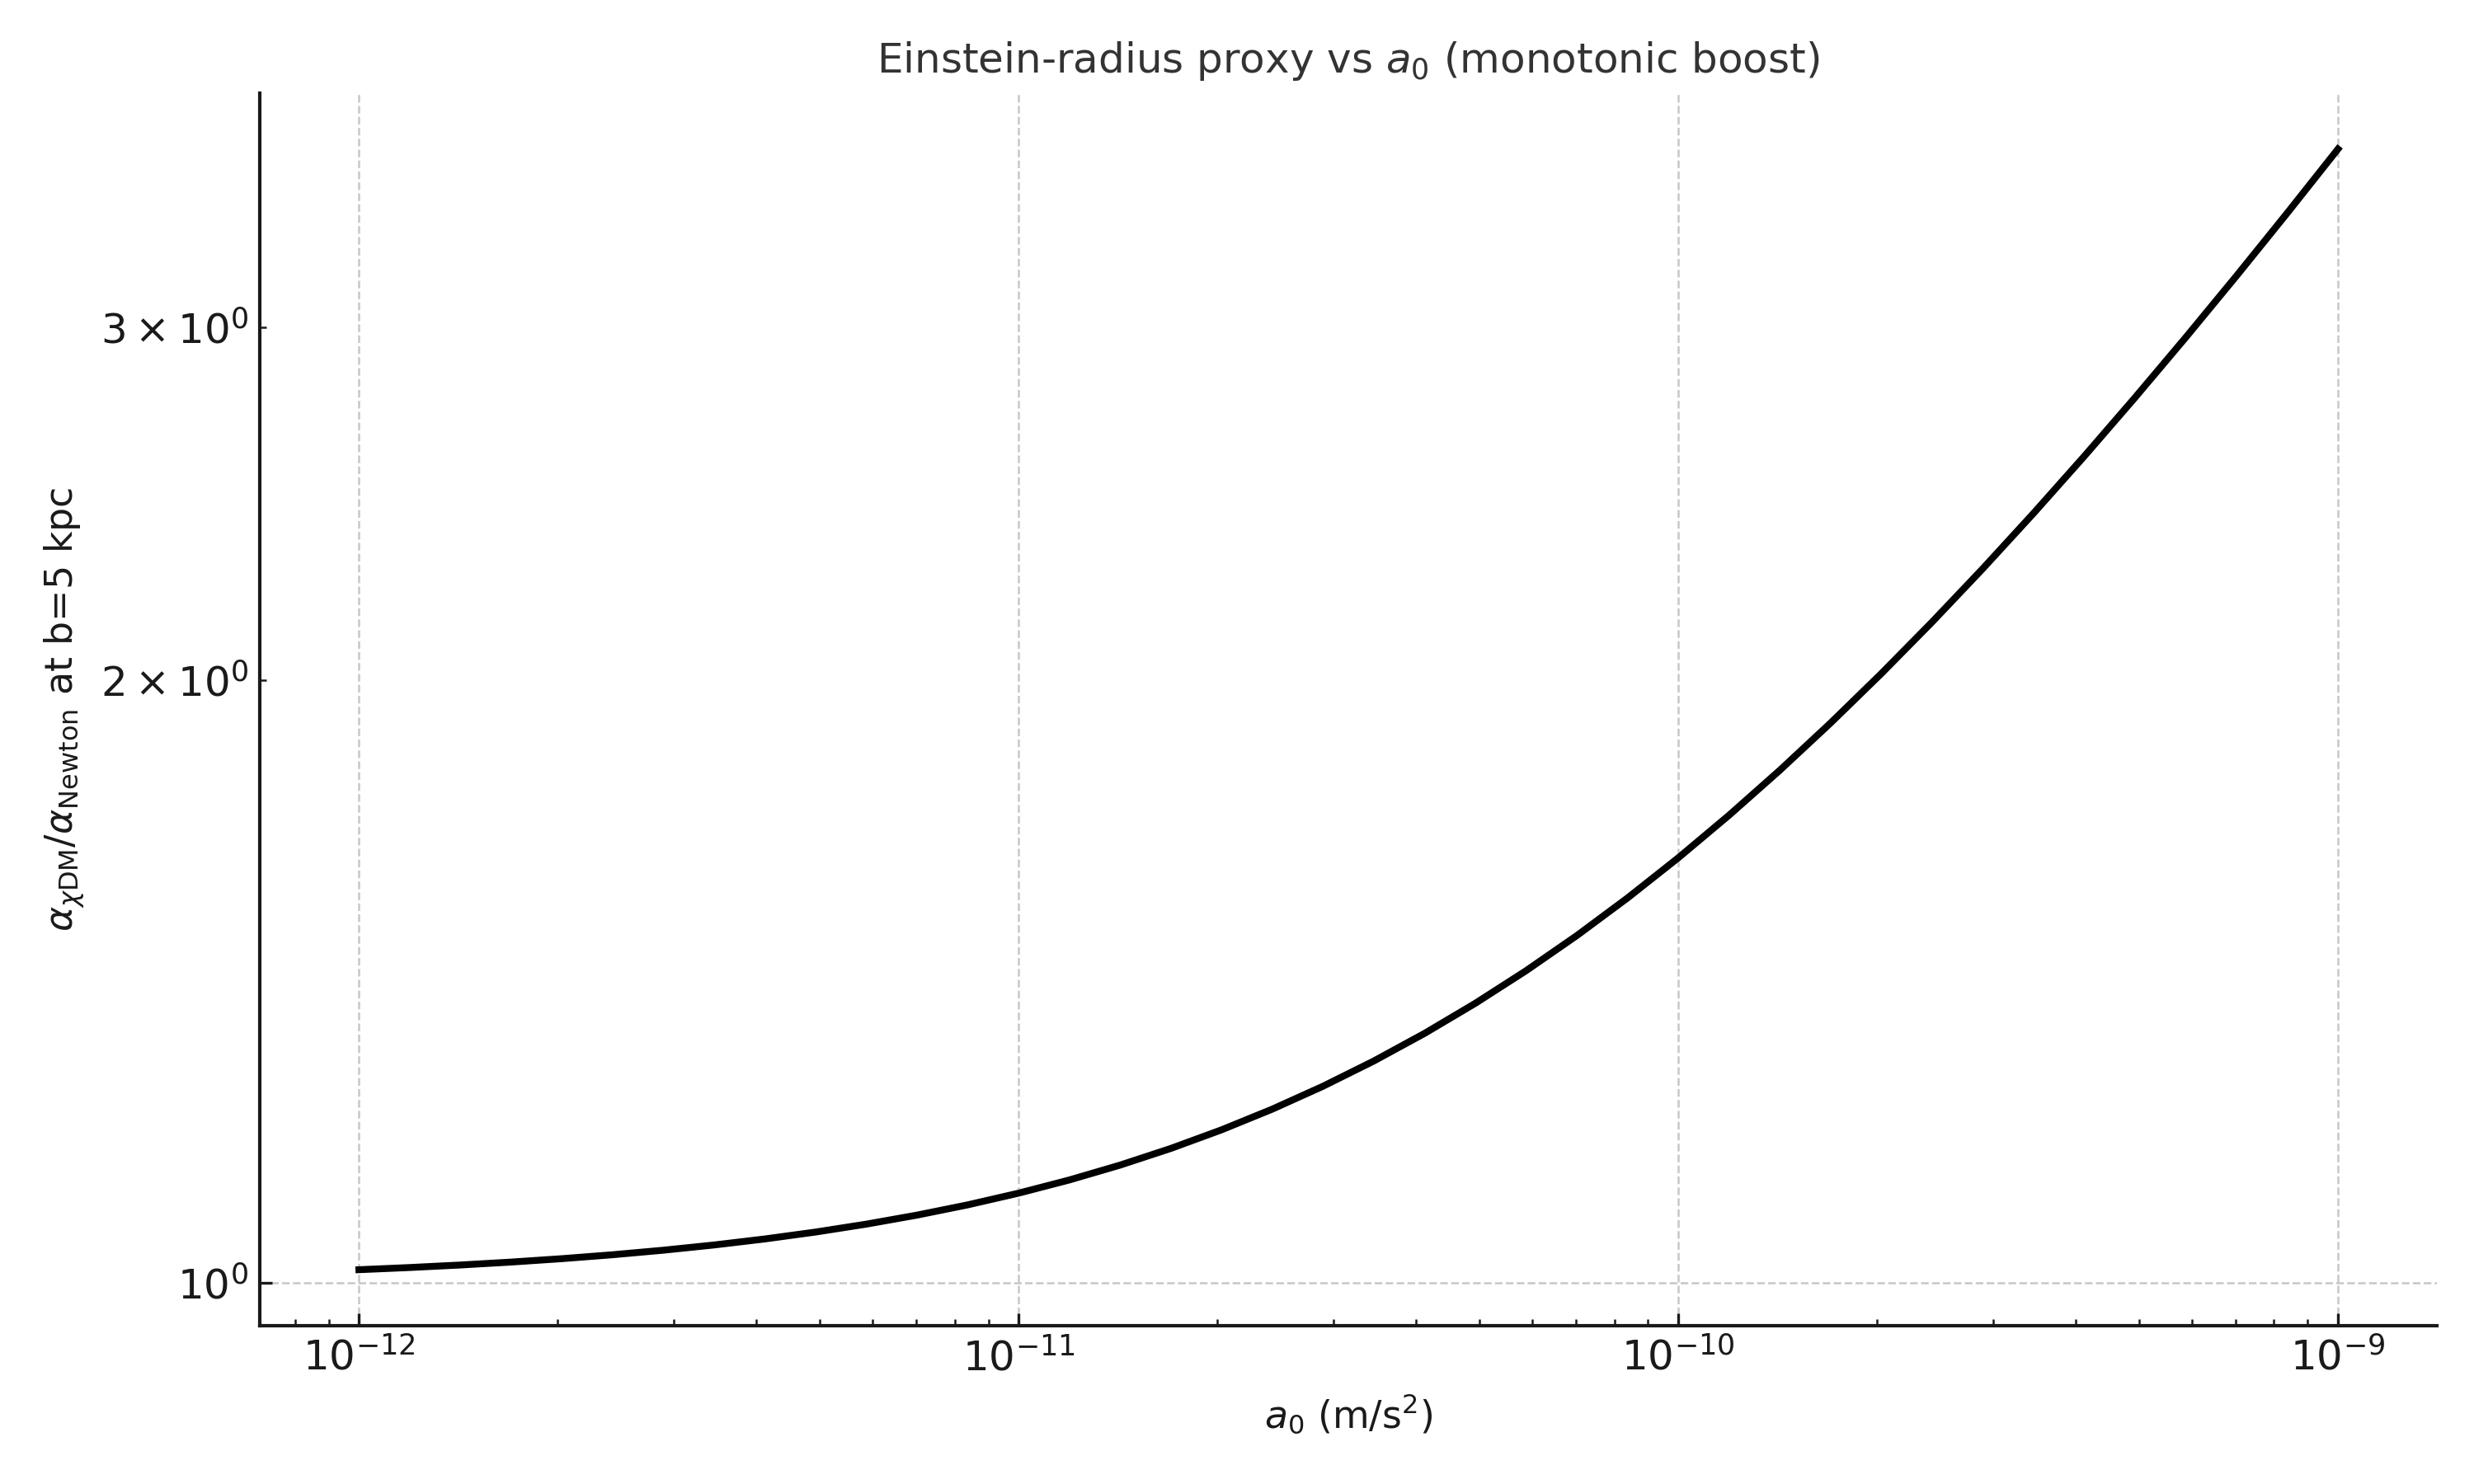
\includegraphics[width=4.78333in,height=2.87in,alt={A graph of a line AI-generated content may be incorrect.}]{letter_media/media/image7.png}

Einstein-radius proxy vs \(\mathbf{a}_{\mathbf{0}}\) (monotonic).
\emph{Definition:} ratio
\(\mathbf{\alpha}_{\mathbf{\chi}\mathbf{DM}}\mathbf{/}\mathbf{\alpha}_{\mathbf{Newton}}\)
at fixed \(\mathbf{b}\mathbf{=}\mathbf{5}\) kpc. Larger
\(\mathbf{a}_{\mathbf{0}}\) increases the deflection in the
low-acceleration regime.

\section{Appendix C: Shapiro delay geometry (near-conjunction
limit)}\label{appendix-c-shapiro-delay-geometry-near-conjunction-limit}

For emitter/receiver distances \(r_{E},r_{R}\) from a point mass \(M\)
and impact parameter \(b \ll r_{E},r_{R}\),

\[\Delta t_{Shapiro} = (1 + \gamma)\frac{GM}{c^{3}}\ln\frac{4r_{E}r_{R}}{b^{2}}\mathcal{+ O}\left( \frac{b}{r_{E,R}} \right).\]

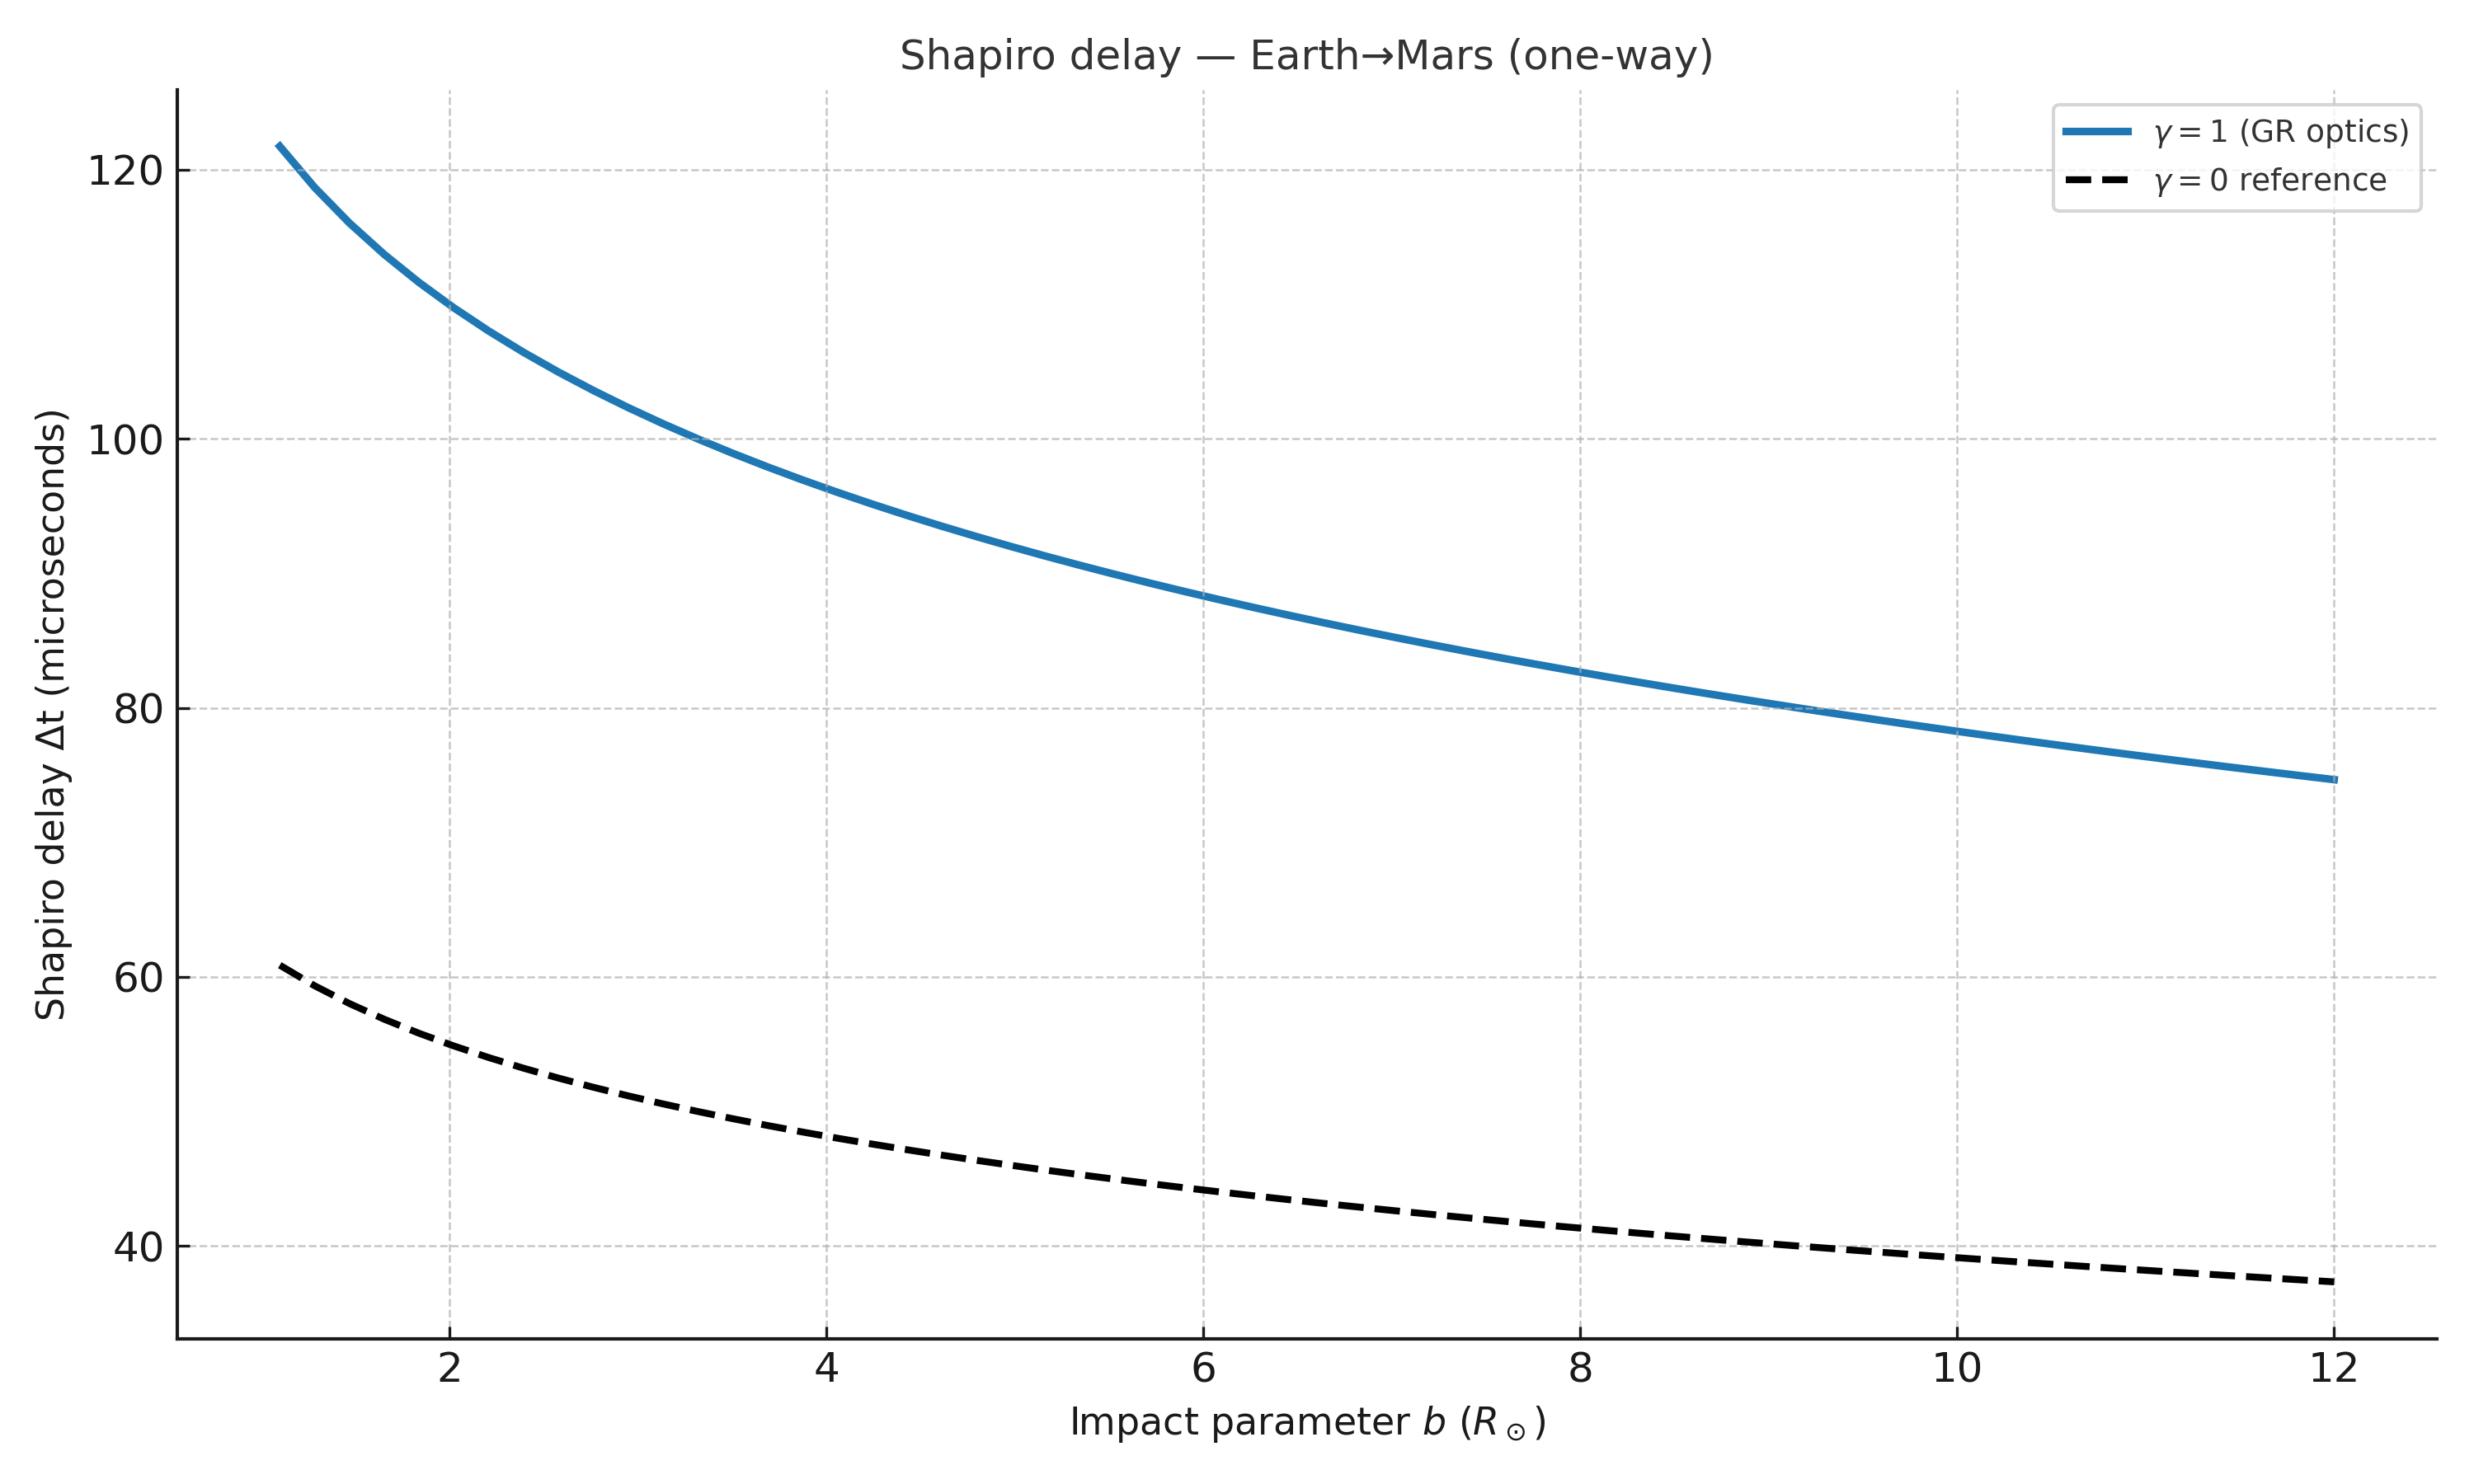
\includegraphics[width=4.78333in,height=2.87in,alt={A graph of a person with a blue line AI-generated content may be incorrect.}]{letter_media/media/image8.png}

Shapiro delay (Earth\(\mathbf{\rightarrow}\)Mars, one-way).
\emph{Sources/assumptions:} point-mass Sun,
\(\mathbf{\gamma}\mathbf{=}\mathbf{1}\) (GR optics) vs a
\(\mathbf{\gamma}\mathbf{=}\mathbf{0}\) reference. The
\(\mathbf{\gamma}\mathbf{=}\mathbf{1}\) curve is plotted first; the
dashed \(\mathbf{\gamma}\mathbf{=}\mathbf{0}\) reference is overlaid
last.

\section{\texorpdfstring{Appendix D: \(\chi\)-DM mapping and closures (A
\& B
explained)}{Appendix D: \textbackslash chi-DM mapping and closures (A \& B explained)}}\label{appendix-d-chi-dm-mapping-and-closures-a-b-explained}

We use the common one-parameter family with \(\mu(y) = y/(1 + y)\),
where \(y = g/a_{0}\) and \(g\) is the total acceleration. The
source-side closure \(g_{b} = \mu(g/a_{0})\, g\) gives the closed form

\[g = \frac{1}{2}\left\lbrack g_{b} + \sqrt{g_{b}^{2} + 4g_{b}a_{0}} \right\rbrack,\]

used in the spherical/axially symmetric checks in this letter. For
general geometries, the mapping is implemented via:\\
\textbf{Option A (QUMOND-style PDE).} Solve
\(\nabla^{2}\Phi_{b} = 4\pi G\rho_{b}\), then compute
\(\nabla^{2}\Phi = \nabla \cdot \lbrack\nu(g_{b}/a_{0})\nabla\Phi_{b}\rbrack\).\\
\textbf{Option B (effective density).} Define
\(\rho_{\chi} = (4\pi G)^{- 1}\nabla \cdot \lbrack(\nu - 1)\nabla\Phi_{b}\rbrack\)
and solve \(\nabla^{2}\Phi = 4\pi G(\rho_{b} + \rho_{\chi})\).\\
Either route yields a scalar, curl-free field with the same \(\Phi\)
used for motion and optics.

\end{document}
